% v2-acmsmall-sample.tex, dated March 6 2012
% This is a sample file for ACM small trim journals
%
% Compilation using 'acmsmall.cls' - version 1.3 (March 2012), Aptara Inc.
% (c) 2010 Association for Computing Machinery (ACM)
%
% Questions/Suggestions/Feedback should be addressed to => "acmtexsupport@aptaracorp.com".
% Users can also go through the FAQs available on the journal's submission webpage.
%
% Steps to compile: latex, bibtex, latex latex
%
% For tracking purposes => this is v1.3 - March 2012

\documentclass[prodmode]{acmsmall} % Aptara syntax

\usepackage{pdfpages}
\usepackage{graphicx}
%\usepackage{cite}
\usepackage{listings}
\lstset{
basicstyle=\small\ttfamily,
columns=flexible,
breaklines=true
}

% Document starts
\begin{document}

% Page heads
\markboth{Evan Bradley}{Bank Marketing Project Report}

% Title portion
\title{Bank Marketing Project Report}
\author{
  EVAN BRADLEY
  \affil{Oakland University}
}

\begin{abstract}
  Telemarketing often requires an immense number of calls to obtain a
  proportionally small number of successful transactions. As such, using
  information about the individual being called can be used to great advantage
  in an effort to make fewer calls while obtaining a majority of the successes
  as calling every available number. In this report a database collected by a
  Portuguese bank on telemarketing is analyzed to determine whether the customer
  will subscribe to a term deposit. With twenty attributes and over
  forty-thousand samples, the data is sufficient for the application of machine
  learning to predict the outcome of a call. By applying a number of different
  machine learning techniques, a model is created which can predict when a call
  will result in a term deposit with reasonable frequency while minimizing the
  number of calls made that do not result in a term deposit.
\end{abstract}

\keywords{Financial technology, Telemarketing, Data mining, Machine learning}

\maketitle

\section{Introduction}
The data analyzed is labeled as the Bank Marketing Data Set, which was collected
from May 2008 to November 2010 from a Portuguese bank, and contains just over
forty-thousand examples and their outcomes, ordered chronologically
\cite{paper}. It was retrieved in a CSV format, where it was then read for
processing and training. Multiple machine learning classifiers were tested with
the data to determine which could produce the desired results, including
k-nearest neighbors, Naive Bayes, neural networks, Support Vector Machines
(SVMs), decision trees, and random forests.

The organization of this paper has been divided into 4 sections: overview of
data, overview of the process used in classification, the application and
results of machine learning, and conclusions based on the results given by the
resulting model. As an overview of the dataset, the variables in the data are
discussed, and relations between them are found. Afterward, a process which was
set up in RapidMiner Studio to pre-process the data and train a classifier on it
is discussed. Multiple classifiers were tried with different options in
preprocessing to obtain a final result. Finally, the conclusions obtained from
the application of the classifiers to the data are discussed for further
research and knowledge discovery.

\section{Overview of Data}
The features in the dataset can be divided into three categories: customer
information, telemarketing campaign information, and economic data. Furthermore,
the features can be divided into nominal and numerical data. The descriptions of
each variable and the type values they hold are described in Table 1.

\begin{table}[!t]
  \tbl{Description of variables and their types. There are 21 variables
  in total, with the y variable being an output variable.}{
  \begin{tabular}{ | c | c | c | }
\hline
    \textbf{Name of variable} & \textbf{Description} & \textbf{Type} \\ \hline
    age & Age in years & Discrete numeric \\ \hline
    job & Field of job & Nominal \\ \hline
    education & Level of education reached & Nominal \\ \hline
    default & Whether the client has credit in default & Nominal \\ \hline
    housing & Whether the client has a housing loan & Nominal \\ \hline
    loan & Whether the client has a personal loan & Nominal \\ \hline
    contact & How the client was contacted & Nominal \\ \hline
    month & Month of contact & Nominal \\ \hline
    day\_of\_week & Day of week of contact & Nominal \\ \hline
    duration & Duration of call & Discrete numeric \\ \hline
    campaign & Number of calls during this campaign & Discrete numeric \\ \hline
    pdays & Number of days since last contact & Discrete numeric \\ \hline
    previous & Number of contacts before this campaign & Discrete numeric \\ \hline
    poutcome & Outcome of previous contact & Nominal \\ \hline
    emp.var.rate & Employment Variation Rate & Continuous numeric \\ \hline
    cons.price.idx & Consumer Price Index & Continuous numeric \\ \hline
    cons.conf.idx & Consumer Confidence Index & Continuous numeric \\ \hline
    euribor3m & Euro Interbank Offered Rate for three months & Continuous numeric \\ \hline
    nr.employed & Number of employees & Discrete numeric \\ \hline
    y & Outcome of this contact & Nominal \\ \hline
  \end{tabular}}
\end{table}

Of important note on basic review of the data is the role of the duration
variable in the dataset and the unbalanced nature of the different classes of y.
The duration variable records the duration of the phone call, and as such is
highly correlative with the output. Furthermore, since it is not known until the
call has ended and subsequently the result is known, it was immediately thrown
out before pre-processing or classification, and only used to benchmark the
classification models used. \\

Summaries of the data also revealed that the data was highly unbalanced: roughly
89\% of contacts did not result in a term deposit, leaving only 11\% of
successful outcomes. This split is likely to induce classifiers to strongly
favor ``no'' responses in their predictions. Since the goal in classifying this
data is to predict ``yes'' outcomes, which are more valuable, this needs to be
addressed in some fashion. This result is not surprising, however, due to the
many variables involved and expected success levels of a telemarketing campaign.

A chi-squared test was performed in R on the categorical variables in relation
to the outcome variable in an attempt to determine whether they correlate with
whether someone makes a term deposit, and therefore would be useful in
predicting the outcome of a call. Most tests resulted in a remarkably low
p-value at $2.2\cdot10^{-16}$, but the personal loan and housing loan variables
had comparatively high p-values, at $0.5787$ and $0.05829$, respectively,
suggesting they do not accurately predict whether a term deposit will be made.

The numerical variables were graphically and numerically analyzed to determine
any obvious patterns they could present. The only variable of note in this
analysis is the comparatively large number of clients who subscribed to a term
deposit if they were contacted multiple times.

\section{Overview of Process}

\begin{figure}[!t]
  \tbl{The overall process used in testing the classifiers.}{
    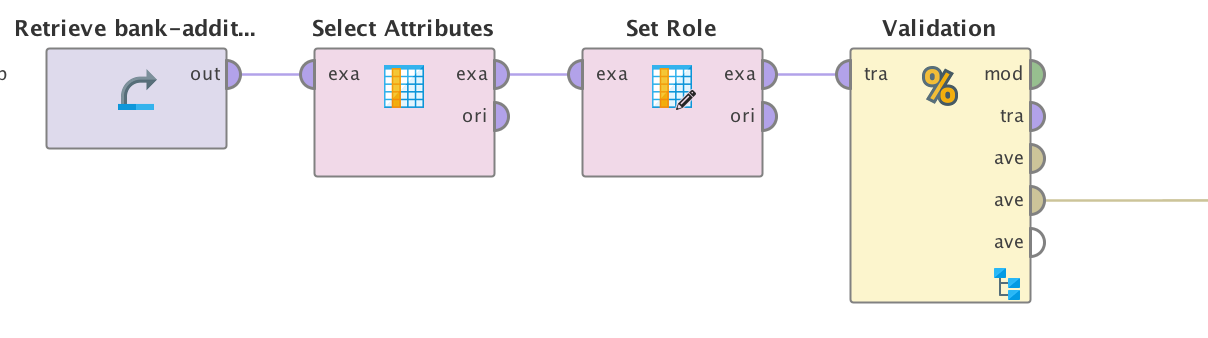
\includegraphics[width = \textwidth]{process}}
\end{figure}

\begin{figure}[!t]
  \tbl{The cross-validation sub-process used to evaluate the model. A random
    forest box is shown here, but could be replaced by any classifier.}{
    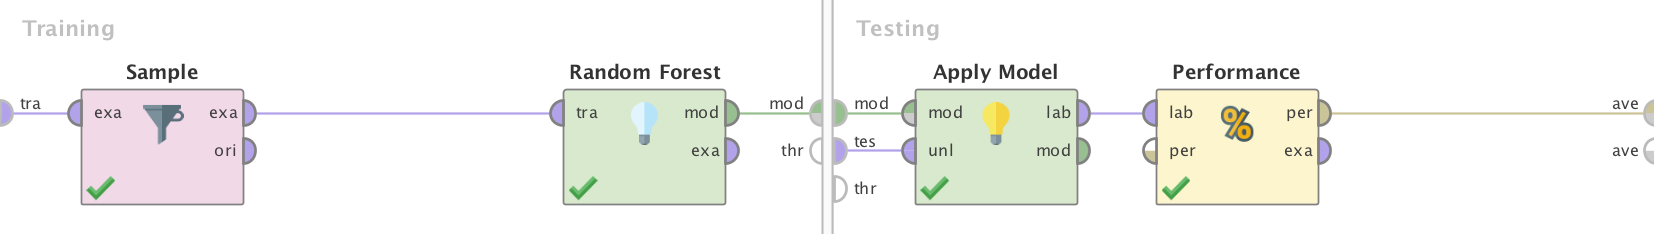
\includegraphics[width = \textwidth]{x-val-process}}
\end{figure}

RapidMiner Studio was used to perform the remainder of the processes that will
be discussed. The process implemented in RapidMiner consists of reading the data
from the full CSV file, performing tests on it to determine its usefulness,
training a classifier on the data, and evaluating the performance of the
classifier and the process as a whole.

After the dataset is read into the process, it is filtered for duration, which
will not be considered in any of the calculations aside from benchmarking. It is
then subsequently split into numeric, economic, and nominal data to be processed
for weighting by importance. Most numeric data is left as is, since there are
not necessarily any tests to determine its importance.

Nominal data was run through another Chi-squared test to determine the weight of
the features in relation to one another, as well as their relationship with the
outcome feature. As determined in the previous test, housing and personal loans
were given very low scores. The rest of the data could be cut off at various
points but mostly had weights between $100$ and $1000$, which were taken to
indicate low to moderate weighting. The month of the contact and the previous
outcome seemed to be incredibly highly correlated with the outcome feature.
 
\begin{figure}[!t]
  \tbl{Graph of the resulting table from the chi-squared test.}{
    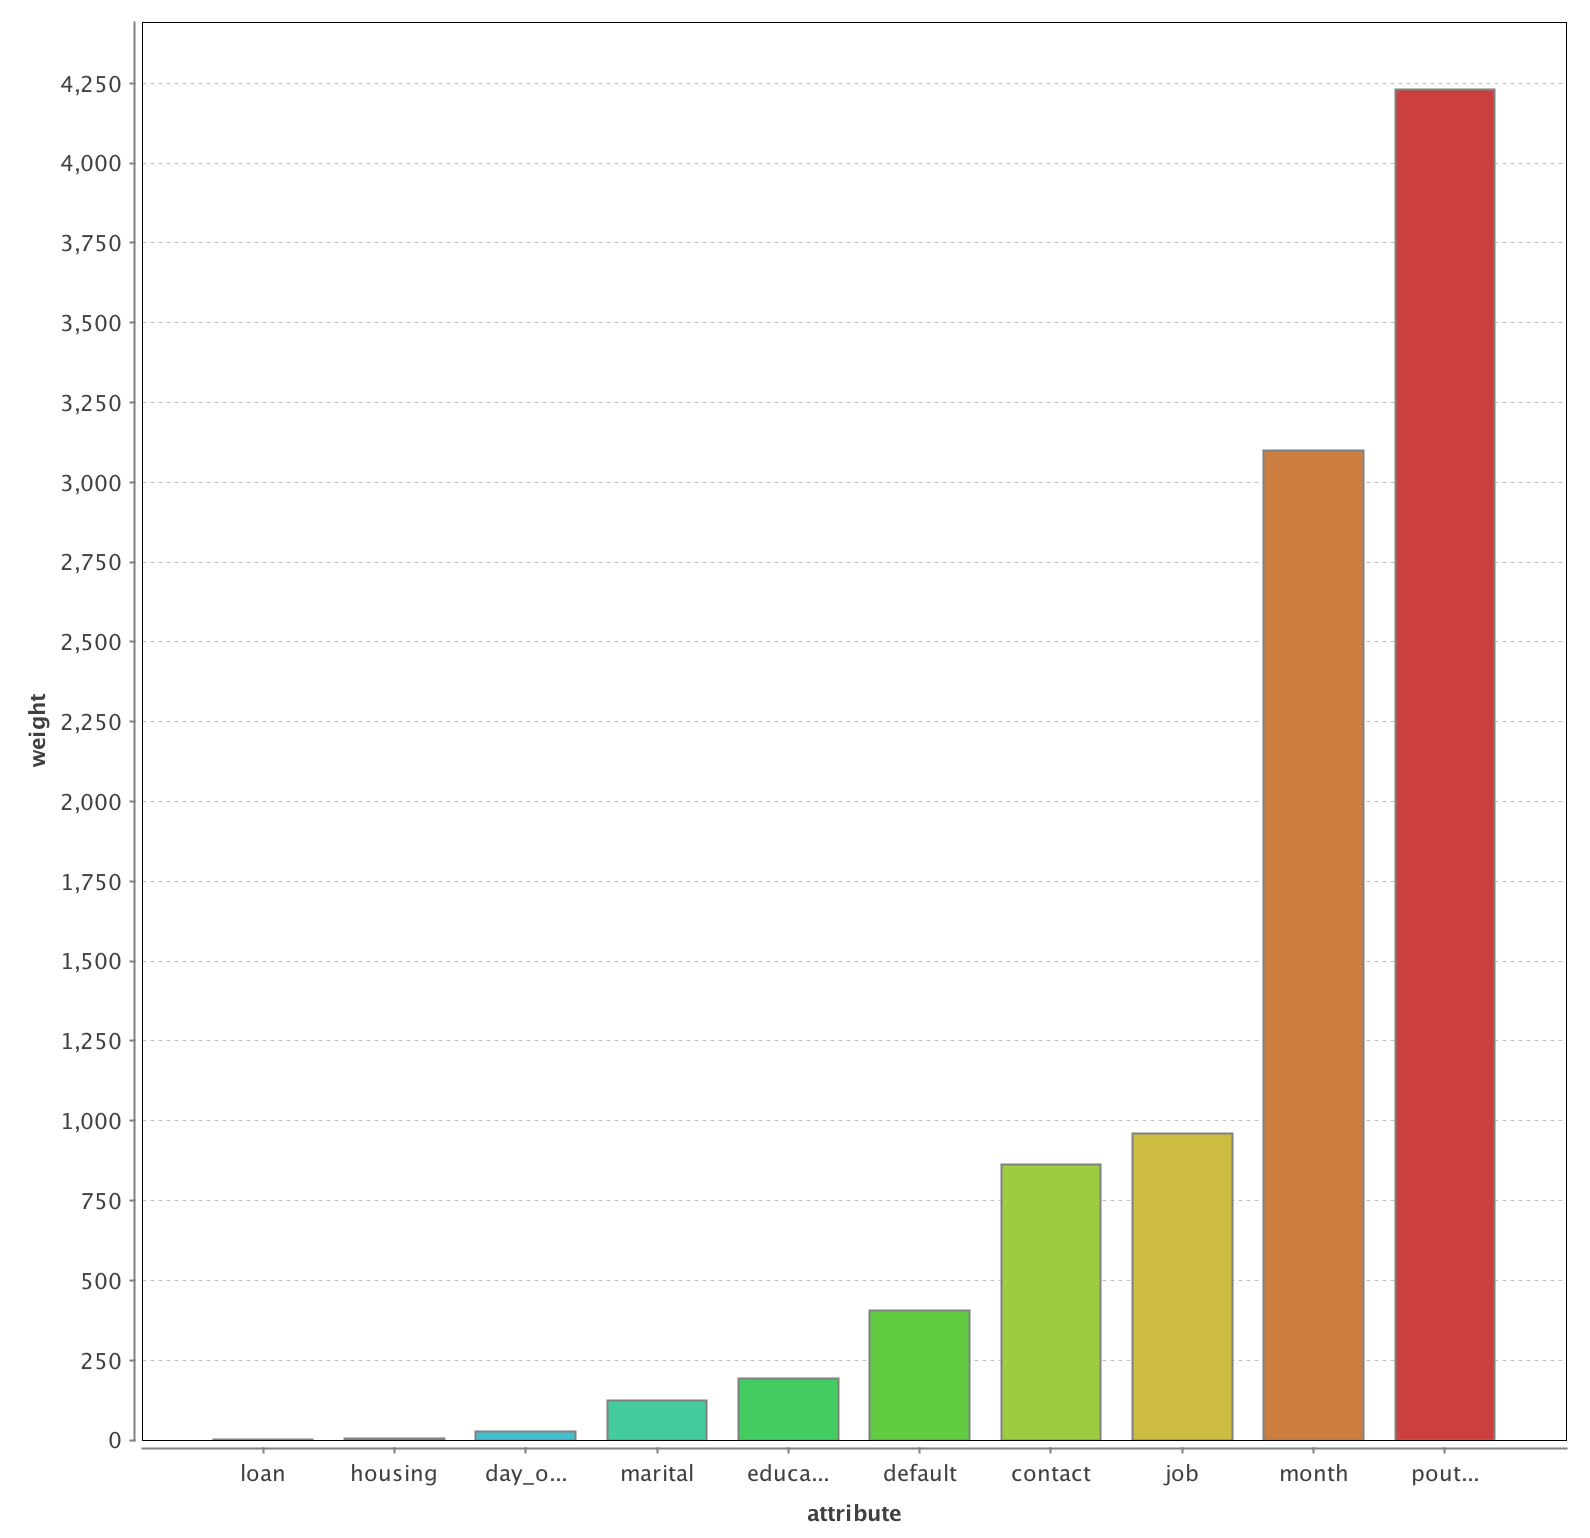
\includegraphics[width = \textwidth]{chi-squared-graph}}
\end{figure}

The economic data would intuitively have many relations as a mechanic of
economic data, so it was run through Principle Components Analysis to determine
where the majority of the variability lies within the data. It was determined
that three of the variables accounted for the majority of the variance, with the
remaining two accounting for enough to be discarded.

\begin{figure}[!t]
  \tbl{Graph of the resulting table from the application of PCA to the economic
    features.}{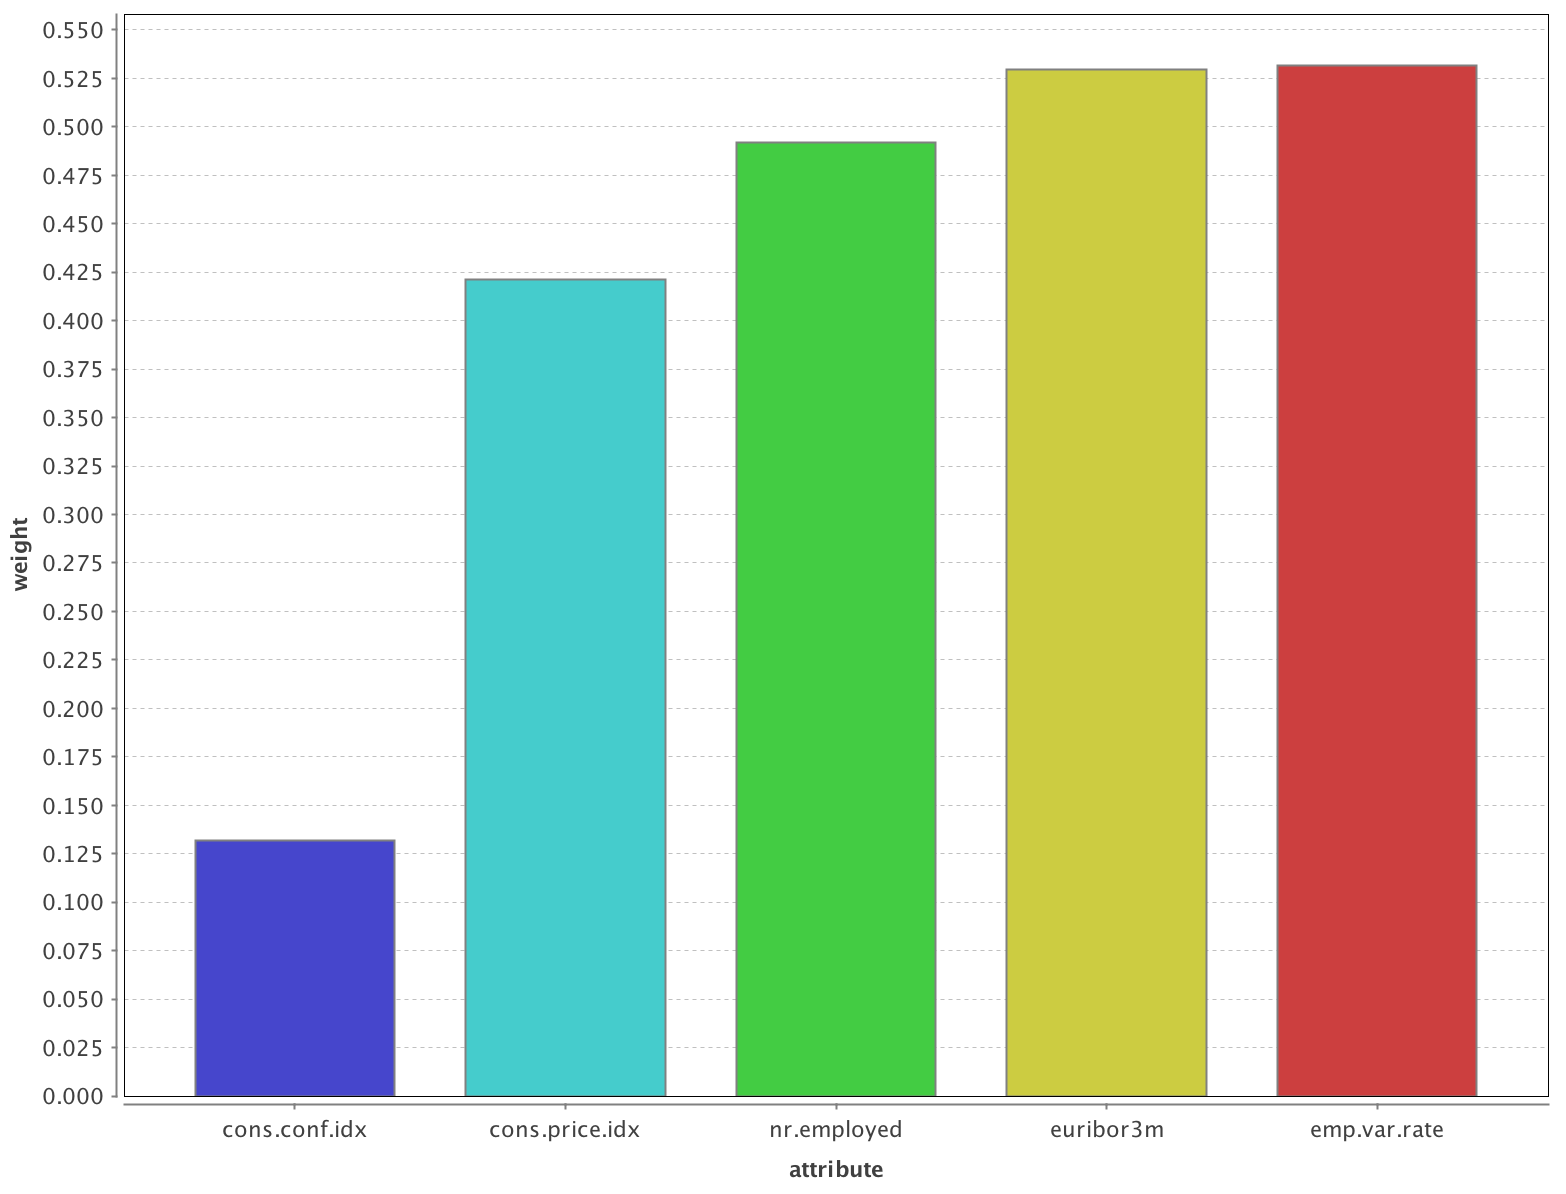
\includegraphics[width = \textwidth]{pca-graph}}
\end{figure}

The remaining numeric data was included in the dataset given to the
classification algorithms without the application of any tests, as it does not
show or suggest any clear relationships that would be of use to PCA and does not
clearly meet the criteria for any other tests.

The selected variables from the chi-squared test and PCA are then chosen from
the original dataset along with the remaining numeric variables for
cross-validation, where the selected classifiers are trained and tested.

\begin{table}[!t]
  \tbl{Table of resulting 13 attributes chosen for use in the training and
    testing datasets, including the output attribute.}{
  \begin{tabular}{ | c | c | c | }
\hline
    \textbf{Name of variable} & \textbf{Description} & \textbf{Type} \\ \hline
    age & Age in years & Discrete numeric \\ \hline
    default & Whether the client has credit in default & Nominal \\ \hline
    contact & How the client was contacted & Nominal \\ \hline
    month & Month of contact & Nominal \\ \hline
    duration & Duration of call & Discrete numeric \\ \hline
    campaign & Number of calls during this campaign & Discrete numeric \\ \hline
    pdays & Number of days since last contact & Discrete numeric \\ \hline
    previous & Number of contacts before this campaign & Discrete numeric \\ \hline
    poutcome & Outcome of previous contact & Nominal \\ \hline
    emp.var.rate & Employment Variation Rate & Continuous numeric \\ \hline
    euribor3m & Euro Interbank Offered Rate for three months & Continuous numeric \\ \hline
    nr.employed & Number of employees & Discrete numeric \\ \hline
    y & Outcome of this contact & Nominal \\ \hline
  \end{tabular}}
\end{table}

Within the cross-validation sub-process, a sample is taken of the portion of the
data chosen by the cross-validation routine for training that equalizes the
number of examples chosen from each output class. Due to the unweighted nature
of the classes within the data, training a classifier will produce results that
favor a ``no'' answer. To combat this, an equal number of elements are chosen
for each class, such that the classifier will produce more even results. To
maximize the training sample, $4260$ elements were taken from the training set
for each class. This is reflective of the number of ``yes'' examples in the
dataset. As a result, the ``yes''-class examples will be over-sampled in the sampling
process, while the ``no''-class examples will be under-sampled.

Finally, the model and data are fed into a performance operator that generates a
confusion matrix and an Area Under the Receiver Operator Characteristic
(AUROC) curve. These are used in conjunction to evaluate the quality of the
classifiers used.

The confusion matrix generated by RapidMiner is a standard confusion matrix,
with the true classes listed on the top of the confusion matrix and the
predicted classes listed on the left of the matrix. The AUROC in RapidMiner
graphs the true-positive rate on the y-axis against the false-positive rate on
the x-axis. The value produced by this curve represents the probability that the
positive class will be ranked higher than the negative class when an example
from each is randomly chosen, with a value of $0.5$ representing the probability
of a random guess. Measuring the ranking of this cost is in line with the goals
of classifying the bank data, where correctly guessing a ``yes'' response is
more valuable than incorrectly guessing a ``no'' response.

\section{Classification}
The bulk of the computation and work performed on the data within the classifier
is performed by the classifier used. As such, multiple classifiers were tested
to determine which would produce the best results. It was found that many of the
classifiers had similar performance, suggesting inherent noise in the data or
the need for more advanced techniques.

\subsection{Decision Tree}
A decision tree was used to produce a baseline for performance of the prediction
model as a value that must be improved on by other classifiers if they are to be
considered effective. It was chosen as a baseline classifier for its
illustration of important attributes and its ability to natively deal with both
categorical and numerical data.

The baseline decision tree included all attributes except duration and did not
perform any sampling to equalize the frequency of each sample. The results it
produced were above a baseline random guess, with an AUC of $.594$. However, it
produced undesired results, only predicting roughly 20\% of the total number of
``yes'' responses.

\begin{table}[!t]
  \tbl{Confusion matrix generated by the decision tree with all attributes and
    no re-sampling.}{
    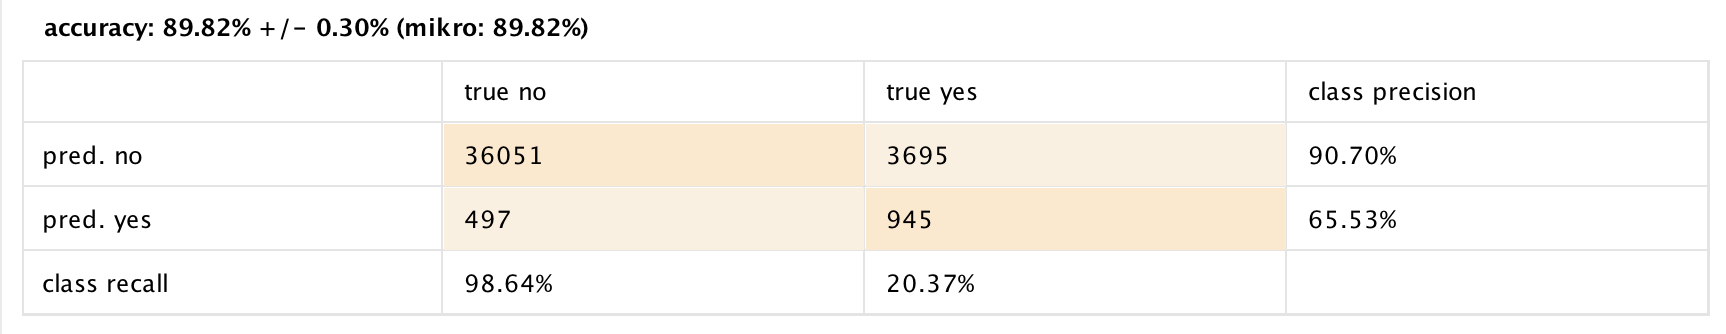
\includegraphics[width = \textwidth]{dt-aa-nos}}
\end{table}

To improve these results, another decision tree was trained on the
restricted set of attributes with class re-sampling applied. This produced much
better results, as nearly half of the ``yes'' responses were accurately predicted,
despite the increase in incorrectly predicted ``no'' responses and accompanying
decrease in the precision of a ``yes'' prediction.  This resulted in a
significant increase in the AUC value to $0.705$.

\begin{table}[!t]
  \tbl{Confusion matrix generated by the decision tree with all attributes and
    no re-sampling.}{
    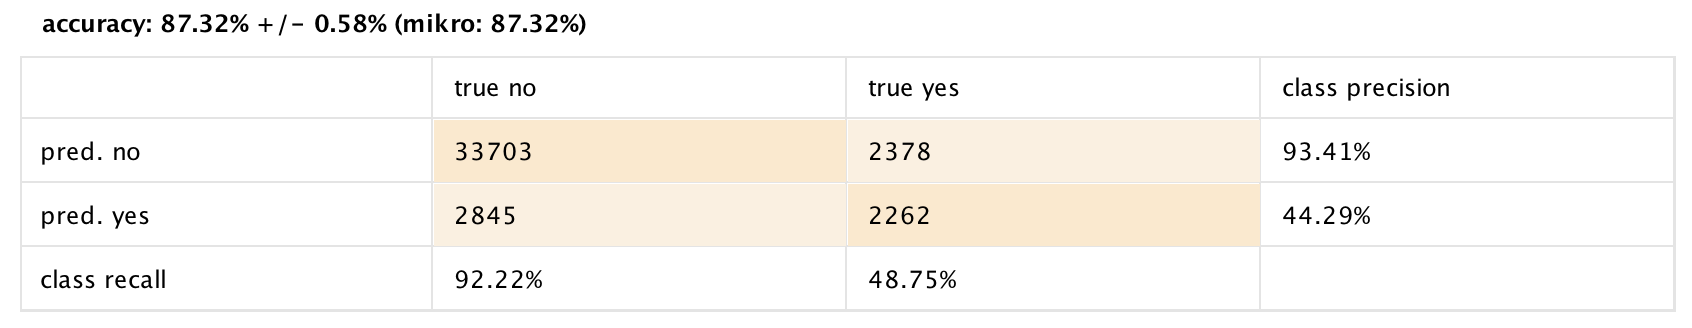
\includegraphics[width = \textwidth]{dt-ra-s}}
\end{table}

From this tree, it can be determined that the economic variables, the customer's
age, and whether the customer was previously contacted appear to have the
greatest influence over whether the customer will subscribe to the term deposit.

\begin{figure}[!t]
  \tbl{A visualization of the decision tree.}{
    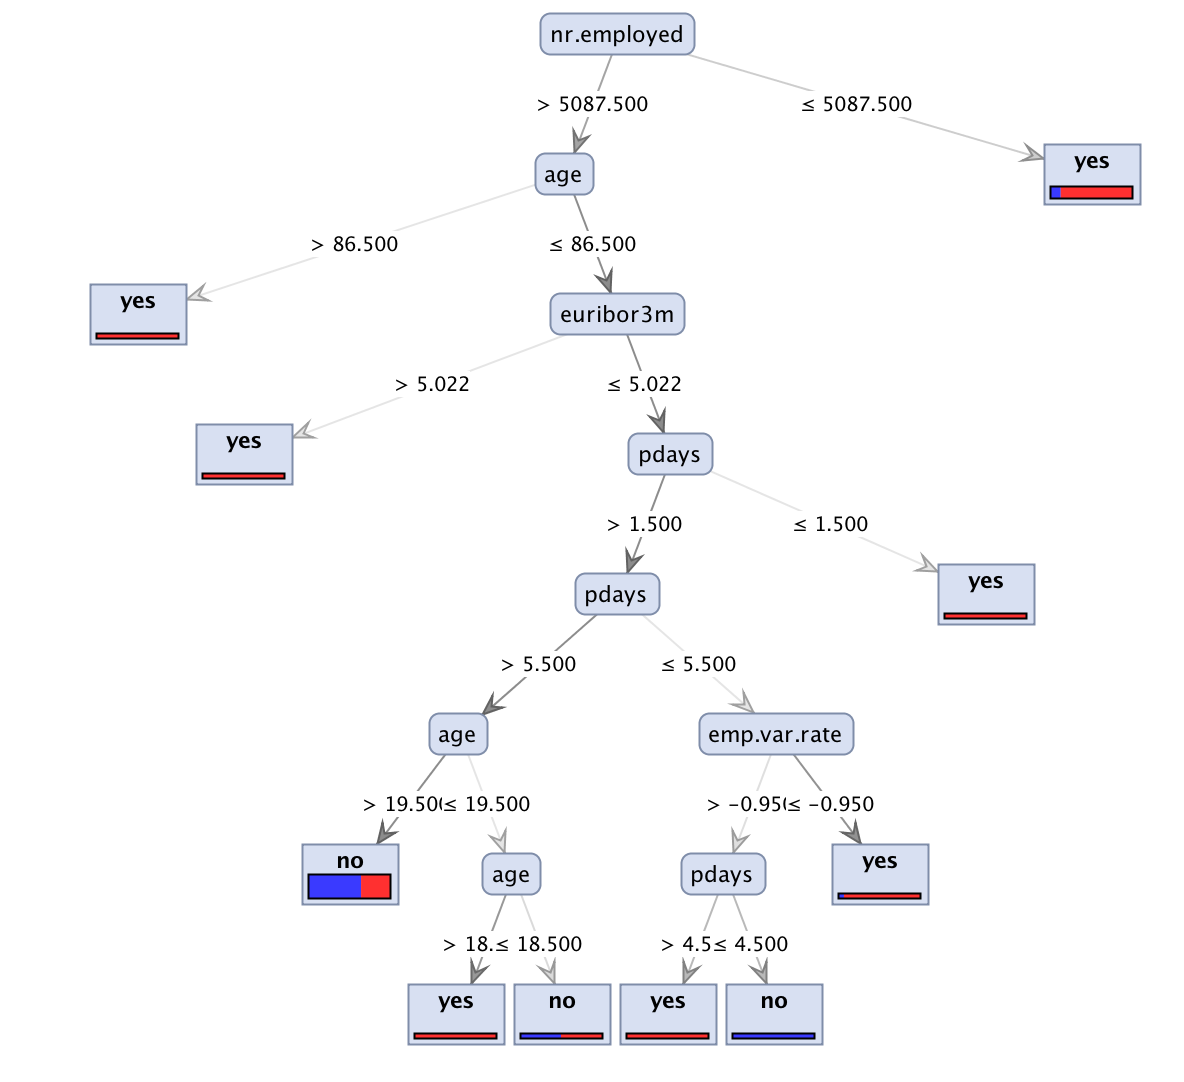
\includegraphics[width = \textwidth]{dt-ra-s-tree}}
\end{figure}

With this baseline established, more sophisticated methods, namely neural
networks, random forests, and SVMs were used to classify the data to determine
the best classification method. Each was trained and tested on the reduced set
of attributes and trained with the reduced sample of equal frequencies for each
class. These methods all produced relatively similar results, indicating a need
for further research in determining the ideal model for the data.

\subsection{Support Vector Machine}
The SVM classifier chosen for use was the standard SVM available in RapidMiner
Studio. Most settings were left as default, with the exception of the kernel
type, which was changed from ``dot'', which is an inner product of two values,
to ``polynomial'', which considers a degree parameter while calculating the dot
product. It was found that a polynomial kernel produced considerably better
results than the dot product, though the value of the degree did not
significantly help if changed from the default value of $2$.

$$\mathrm{k(x,y)} = x \cdot y$$
$$\mathrm{k(x,y)} = (x \cdot y + 1)^d$$ \\

The SVM trained in cross-validation produced noticeably better results than the
decision tree, with a higher recall rate for ``yes'' of just over 60\% and an
AUC of $0.778$. Precision for ``yes'' results similarly lowered to nearly 37\%,
which is lower than the baseline decision tree.

\begin{table}[!t]
  \tbl{The confusion matrix produced from the cross validation of the SVM.}{
    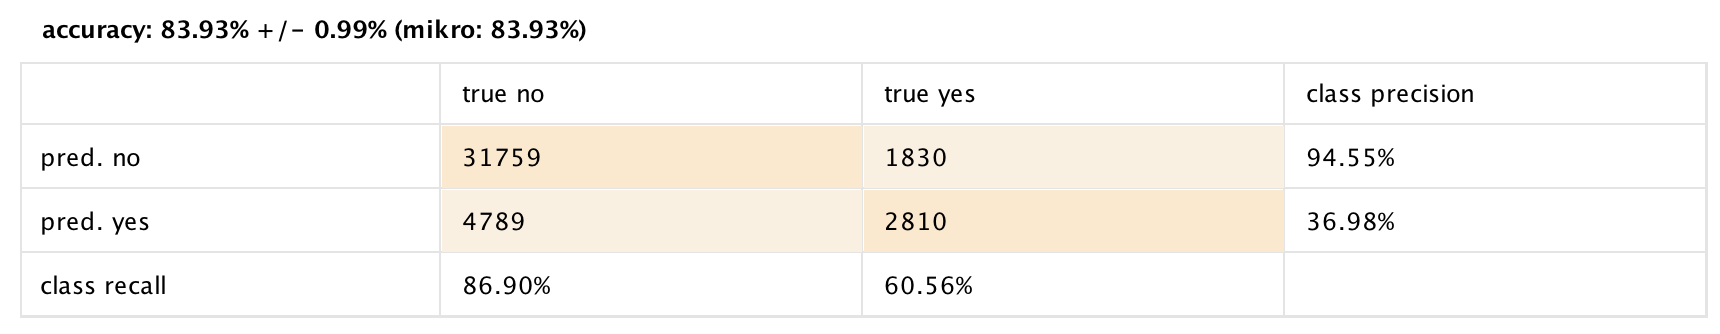
\includegraphics[width = \textwidth]{svm}}
\end{table}

\subsection{Neural Network}
A neural network was then trained on the data and provided reasonable
improvements over the SVM, reaching the rough limit of accuracy obtained in
experimentation. The recall of the ``yes'' responses increased to approximately
61\% with an appropriate increase in the value of the AUC to $0.792$. Modifying
the configuration of the neural network did not produce noticeably better
results, and as such they were left largely similar to the default values.

\begin{table}[!t]
  \tbl{Confusion matrix produced by the neural network.}{
    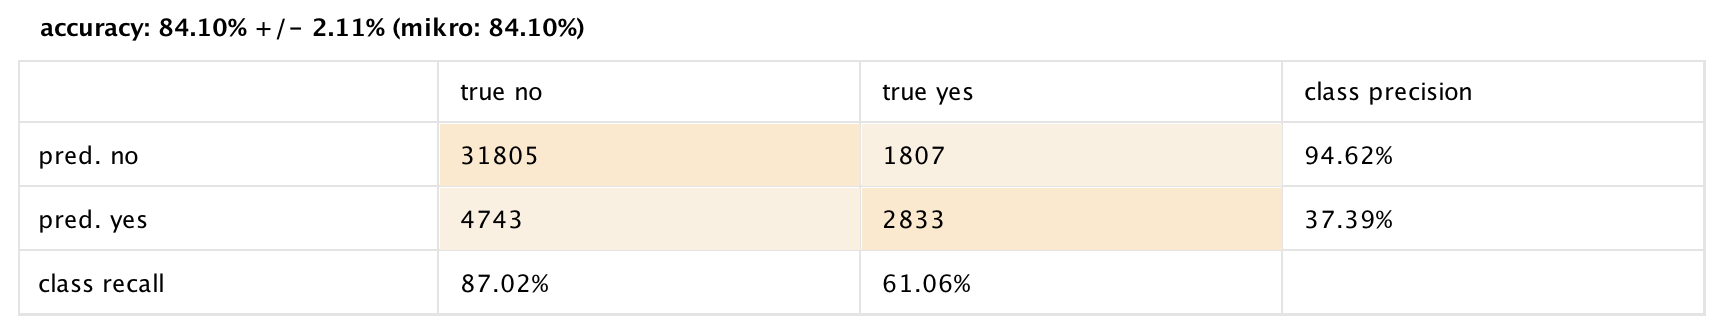
\includegraphics[width = \textwidth]{nn}}
\end{table}

\subsection{Random Forest}
Finally, a random forest was trained on the data, giving the best results seen,
though not significantly better than those obtained by the neural network. The
most substantial modifications to the parameters of the random forest were
increasing the number of trees to 80 and changing the criterion function from a
gain ratio criterion function to the Gini index criterion function. Smaller, but
still significant changes included removing both pre- and post-pruning on the
trees in the random forest and decreasing the tree depth from 20 to 10. These
configurations produced a recall rate of just under 63\% and an AUC of $0.796$.

\begin{table}[!t]
  \tbl{Confusion matrix produced by the random forest.}{
    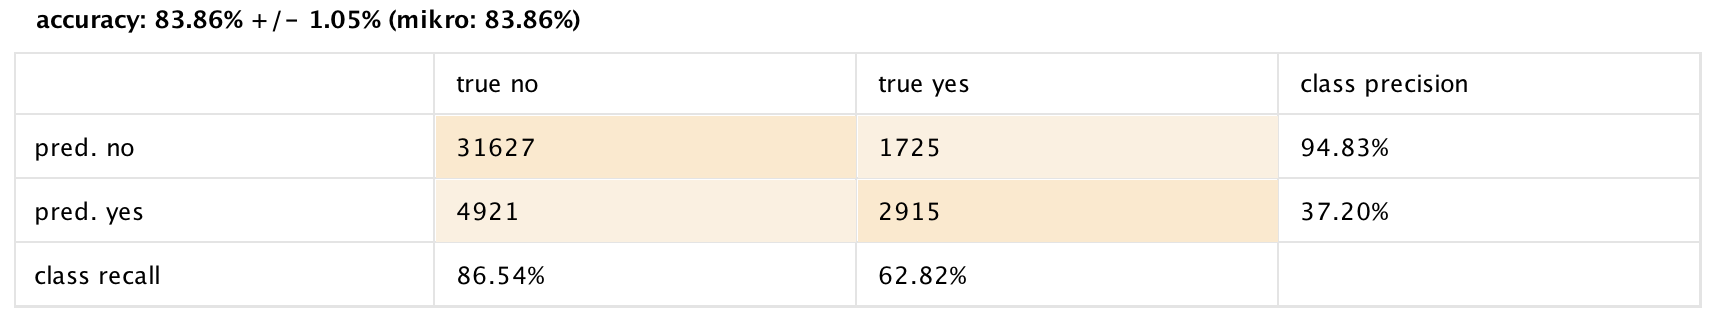
\includegraphics[width = \textwidth]{rf}}
\end{table}

\section{Conclusions}
The results provided by the final prediction model are favorable, though not
optimal, and provide some modest insights into the data. Looking at a small
sample of trees in the generated random forest, it would appear that the
economic and telemarketing campaign features are very important for determining
the outcome due to the frequency in which they appear in the trees. The root
cause of this is difficult to determine, but may be either due to a truly strong
correlation between these attributes and the outcome, an issue in the random
forest algorithm implemented, or in the way in which sampling is performed.

The results suggested by the confusion matrix generated from the random forest
predictions suggest that roughly $\frac{2}{3}$ of the subscribed deposits can be
obtained from calling approximately $\frac{1}{4}$ of the customers available in
the calling pool. Assuming this would carry over for a larger pool of customers,
this model could be applied to a set of 160,000 customers and predict ``yes''
for a fourth of them, coming out to roughly 40,000 calls total, equal to the
number in this dataset. From this, $\frac{2}{3}$ of those called would answer
``yes'' according to the prediction, giving a net gain of $\frac{8}{3}$ term
deposits. Experimentation suggests this ratio could be adjusted to include more
``yes'' responses at the cost of substantially more ``no'' responses, which may
be cost-effective depending on the cost of each call.

Plotting the ignored duration variable can provide insights as to the relative
costs of a call under each class. Plotting duration for each class suggests that
calls resulting in ``no'' responses are typically shorter than those for ``yes''
responses, suggesting that a higher false-positive rate may be acceptable when
considering prediction models. The actual cost of this model would need to be
determined by the institution performing the calls, who would know the costs
induced by each call.

While these results are generally favorable, the limitation reached by the
random forest and neural network classifiers suggests that more research is
needed to determine the optimal model achievable with this data. In an attempt
to break this barrier, numerous methods were tried with little success.

One technique involved splitting the variables into numerical variables and
categorical variables before applying a number of classification models such as
k-Nearest Neighbors, Na{\"i}ve Bayes, and variants on the neural network model
in addition to the three classifiers discussed earlier. This did not produce
significantly better results for any of the classifiers, and as such was not
pursued further. Ensemble methods were also attempted, though more briefly, and
similarly did not produce any results significantly better than what was
achieved with the use of random forests and neural networks.

Since these models did not produce better results, random forests were
considered to be the current best model for their simplicity and speed in
application. This does not necessarily imply that more advanced techniques will
not yield better results, however. Both bagging and boosting could produce
better results through better application of weaker classifiers, and a better
sampling method may assist in reducing the false-positive rate by creating
artificial ``yes'' examples rather than sharply reducing the ``no'' samples used
in training.

It is similarly possible that the data provided does not offer enough
information to produce a more accurate model. The dataset used in \cite{paper}, where an
AUC of $0.929$ was achieved, contained 85 attributes before dimensionality
reduction, and as such may have provided features which better predicted the
data than the features included in the dataset provided for public use.

While there is considerably more area for further research, the results given by
the predictive model constructed with the random forest classifier are
sufficient to improve telemarketing efficiency for this data, under the
assumption that time is a constraint in performing calls. 

\bibliographystyle{acm}
\bibliography{references}
% \section{References}
% S. Moro, P. Cortez and P. Rita. A Data-Driven Approach to Predict the Success
% of Bank Telemarketing. Decision Support Systems, Elsevier, 62:22-31, June 2014

\section{Appendix}
Below are the duration graphs, the AUROC graphs and configurations for each
classifier used, and portions of samples from the random forest trees.
\newpage

\begin{figure}[!t]
  \tbl{A histogram and box-plot of duration for each class to visualize its
    variance between each class of response}{
    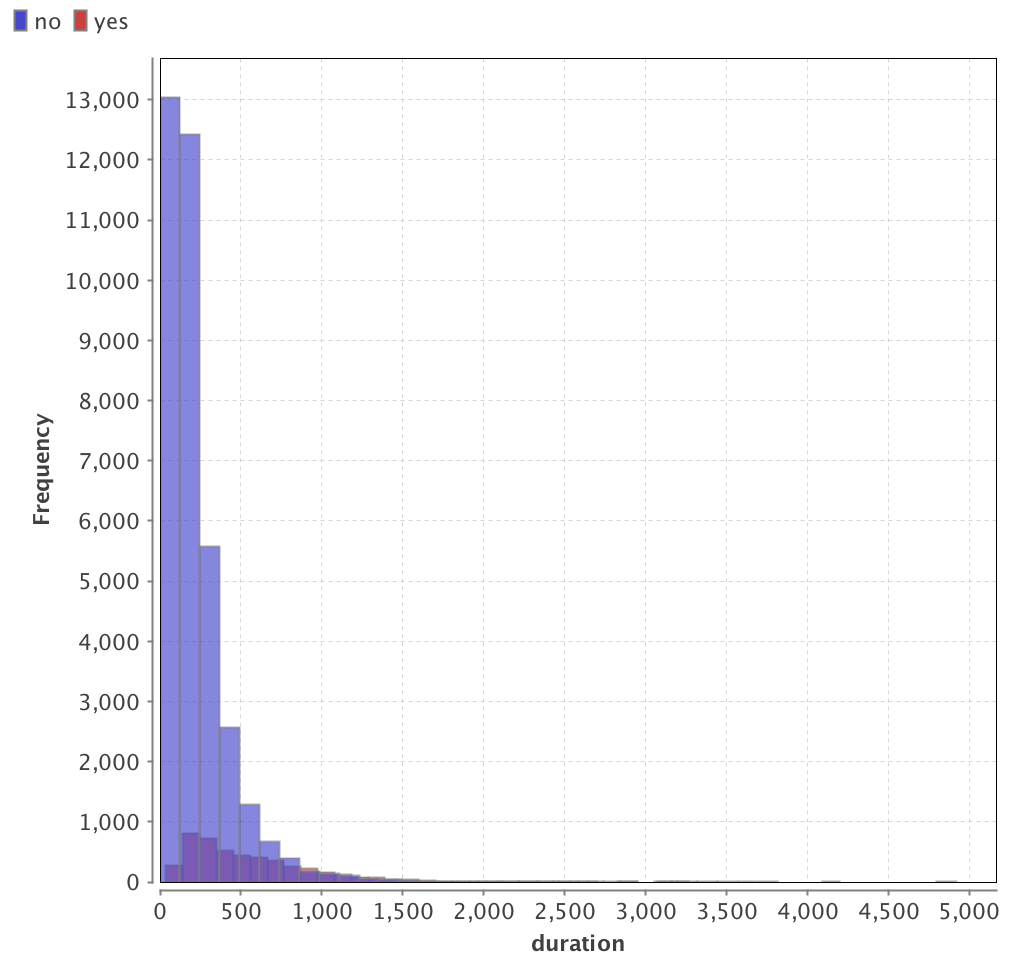
\includegraphics[width = \textwidth]{duration-histogram}}
\end{figure}

\begin{figure}[!t]
  \tbl{A histogram and box-plot of duration for each class to visualize its
    variance between each class of response}{
    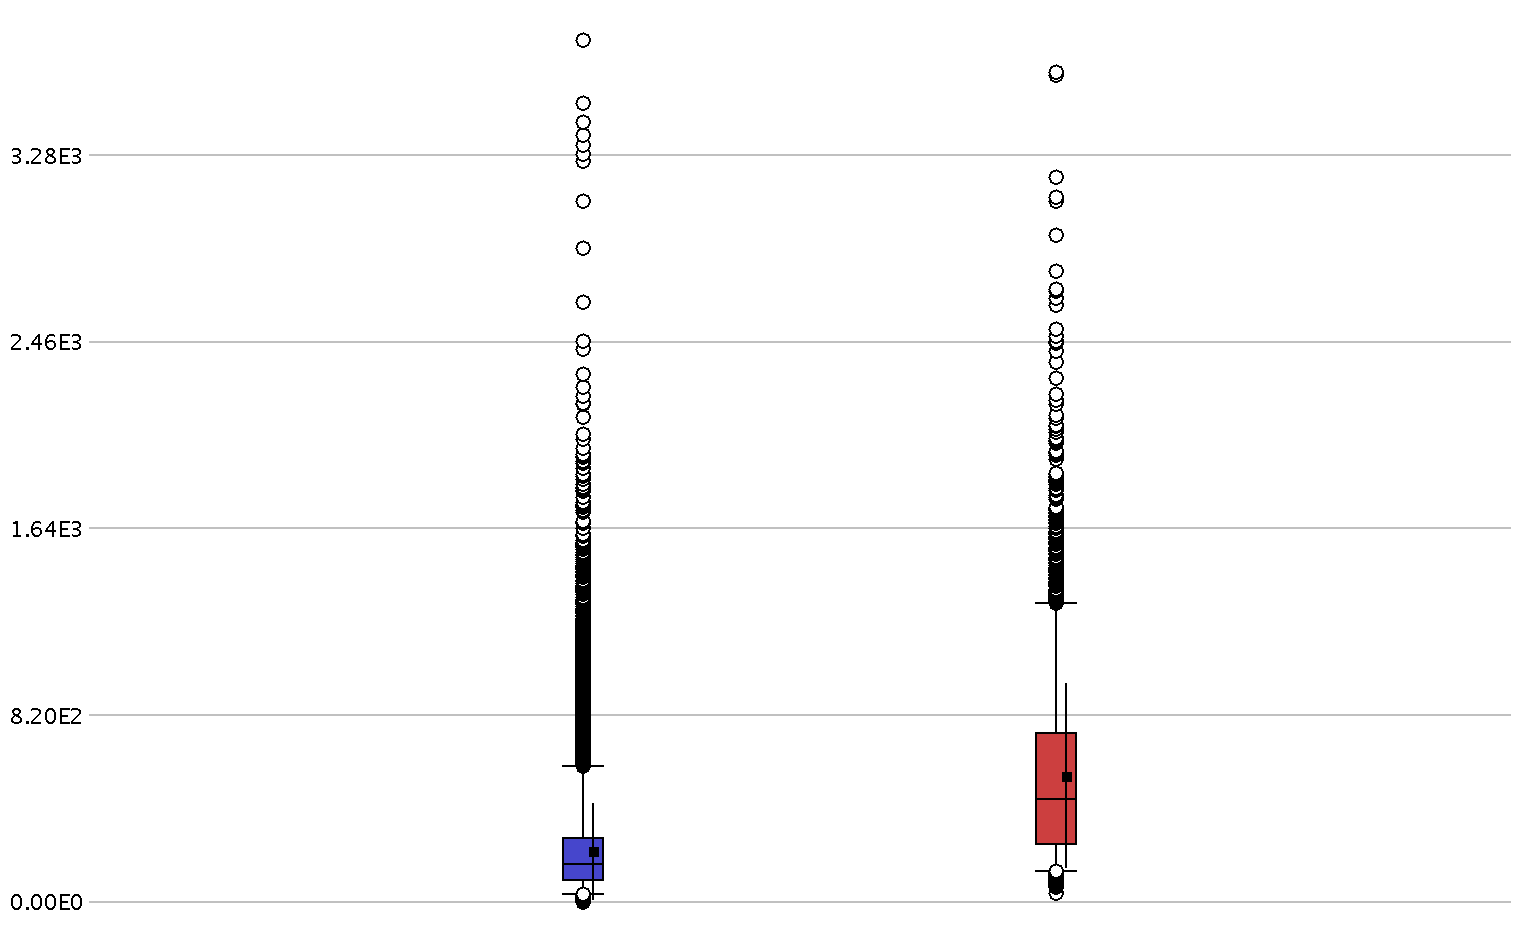
\includegraphics[width = \textwidth]{duration-boxplot}}
\end{figure}

\begin{figure}[!t]
  \tbl{AUROC for the decision tree with all attributes and no re-sampling.}{
    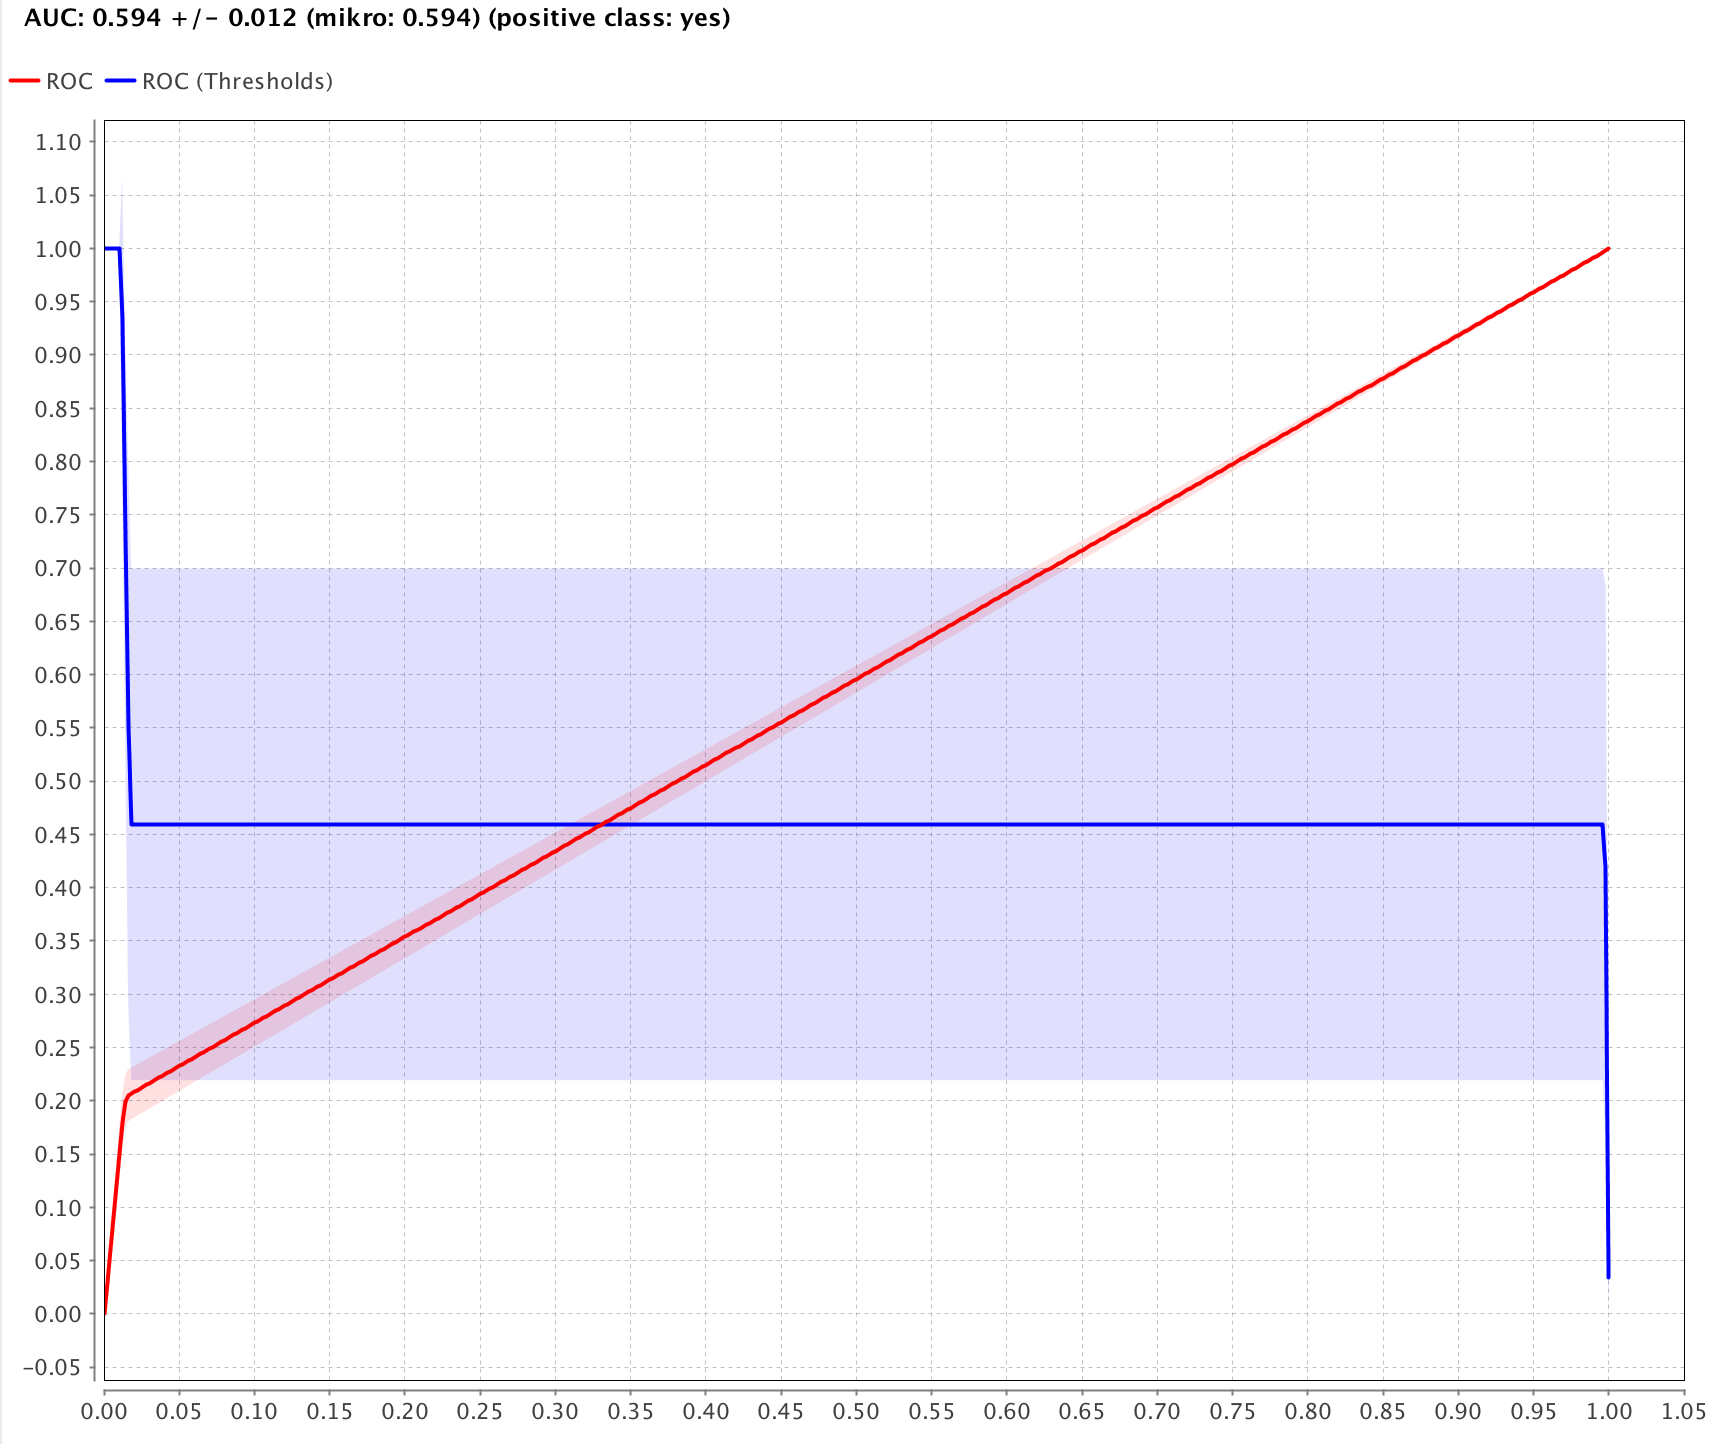
\includegraphics[width = \textwidth, height = 0.4\textheight, keepaspectratio]{dt-aa-roc}}
\end{figure}

\begin{figure}[!t]
  \tbl{AUROC for the decision tree with restricted attributes and re-sampling.}{
    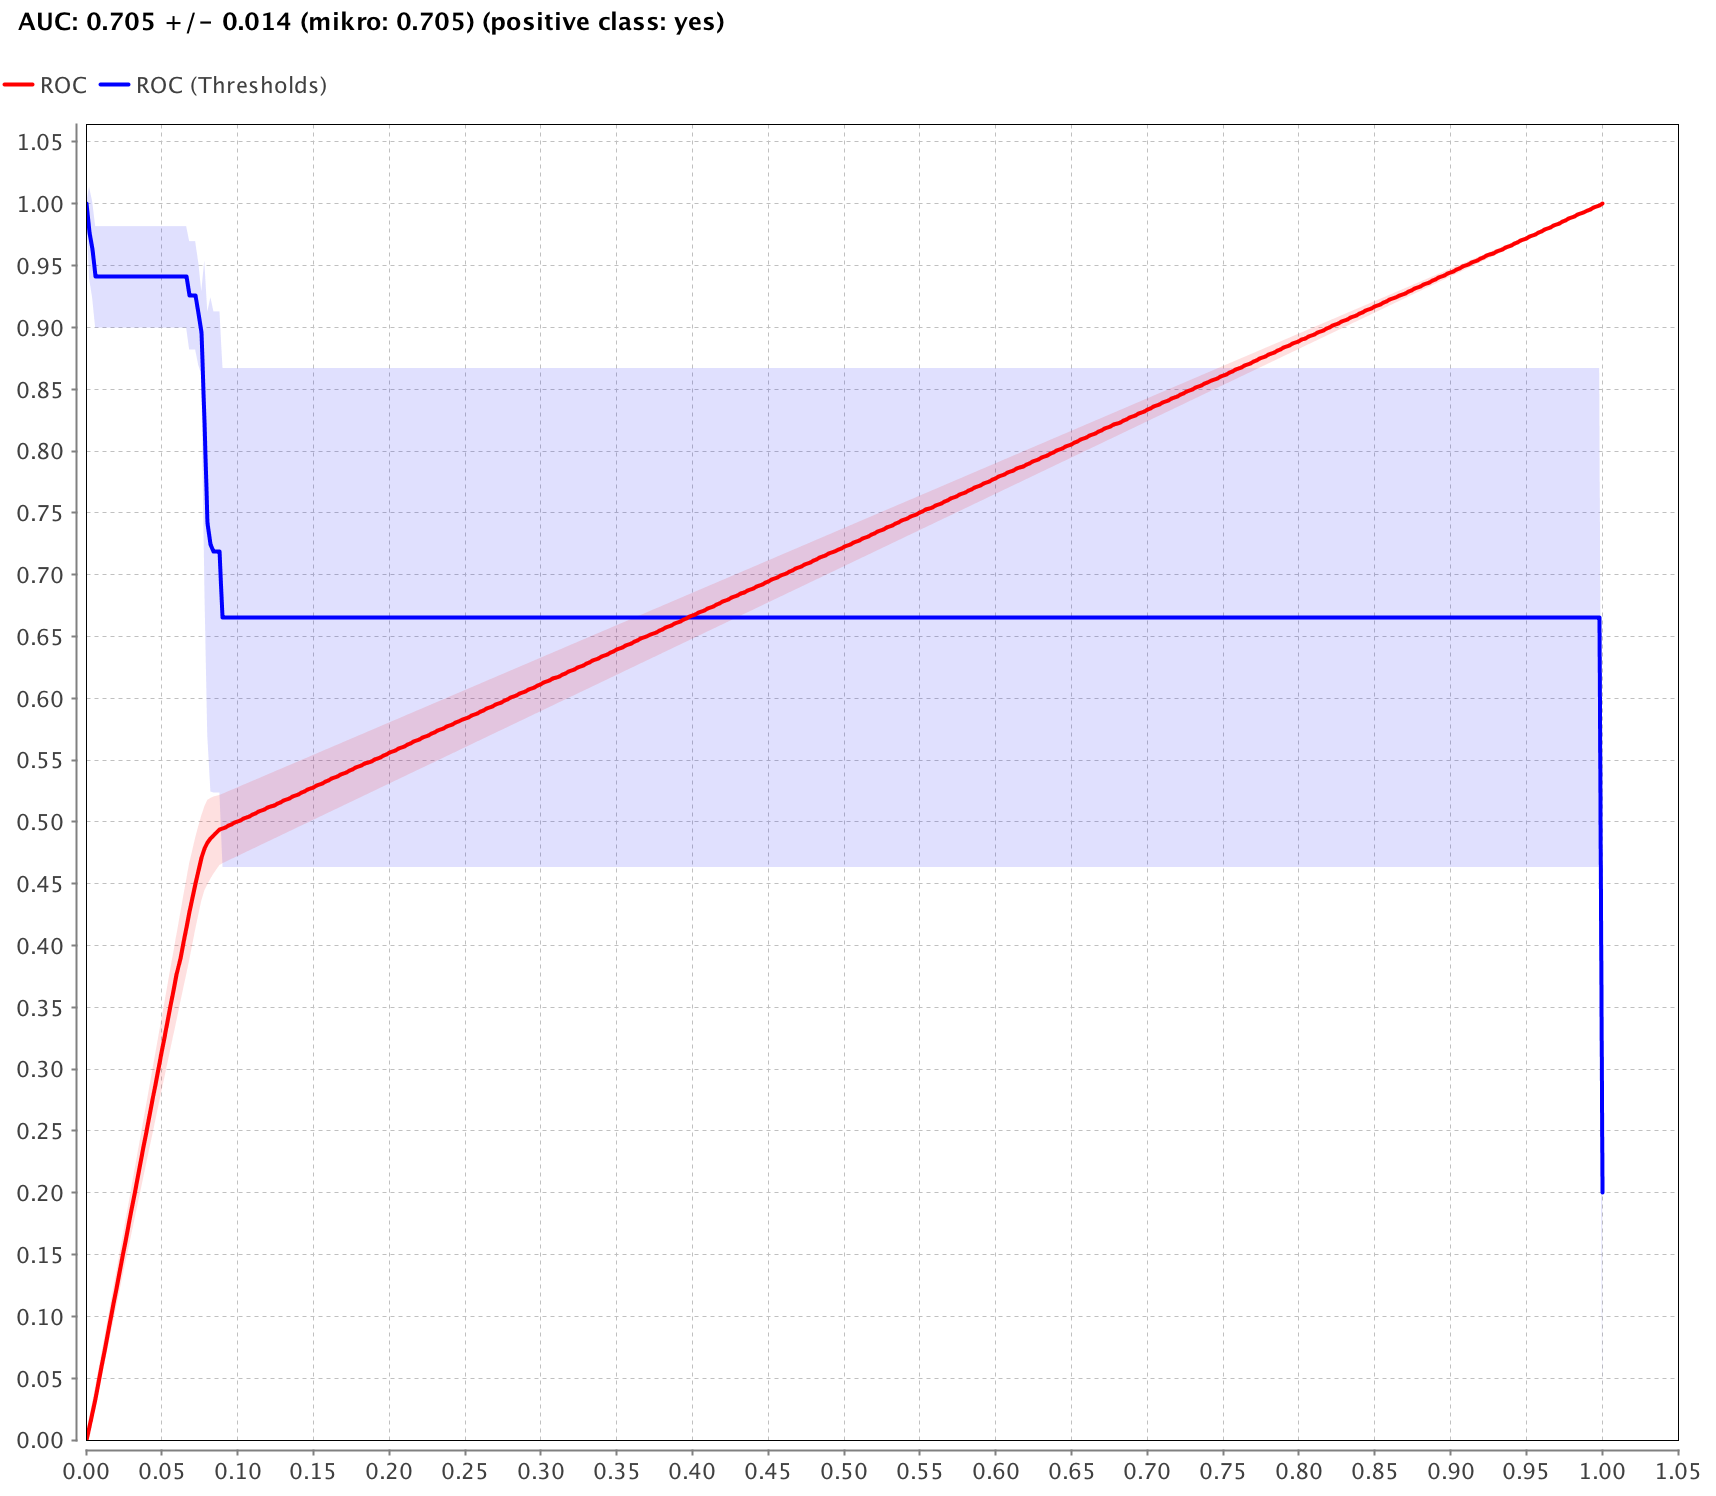
\includegraphics[width = \textwidth, height = 0.4\textheight, keepaspectratio]{dt-ra-s-roc}}
\end{figure}

\begin{figure}[!t]
  \tbl{Options used in configuring the SVM.}{
    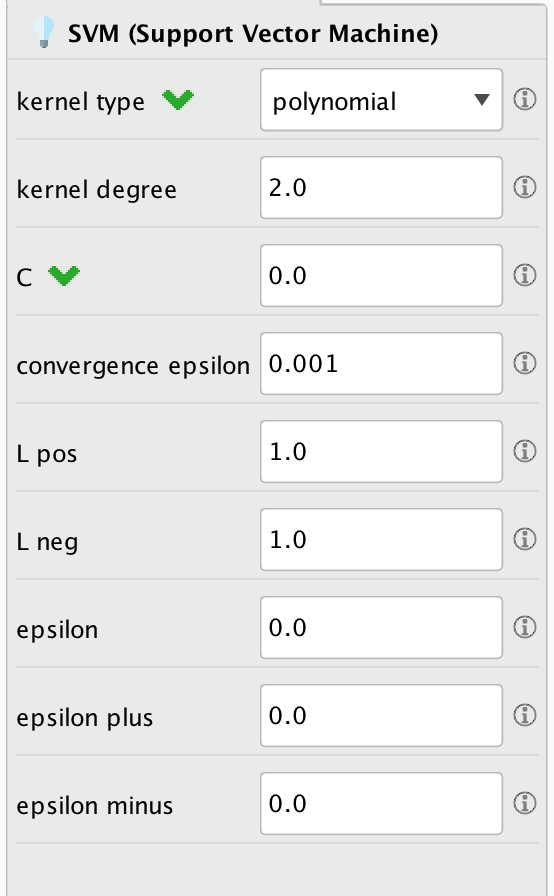
\includegraphics[width = \textwidth, height = 0.4\textheight, keepaspectratio]{svm-opt}}
\end{figure}

\begin{figure}[!t]
  \tbl{AUROC for the predictions made by the SVM.}{
    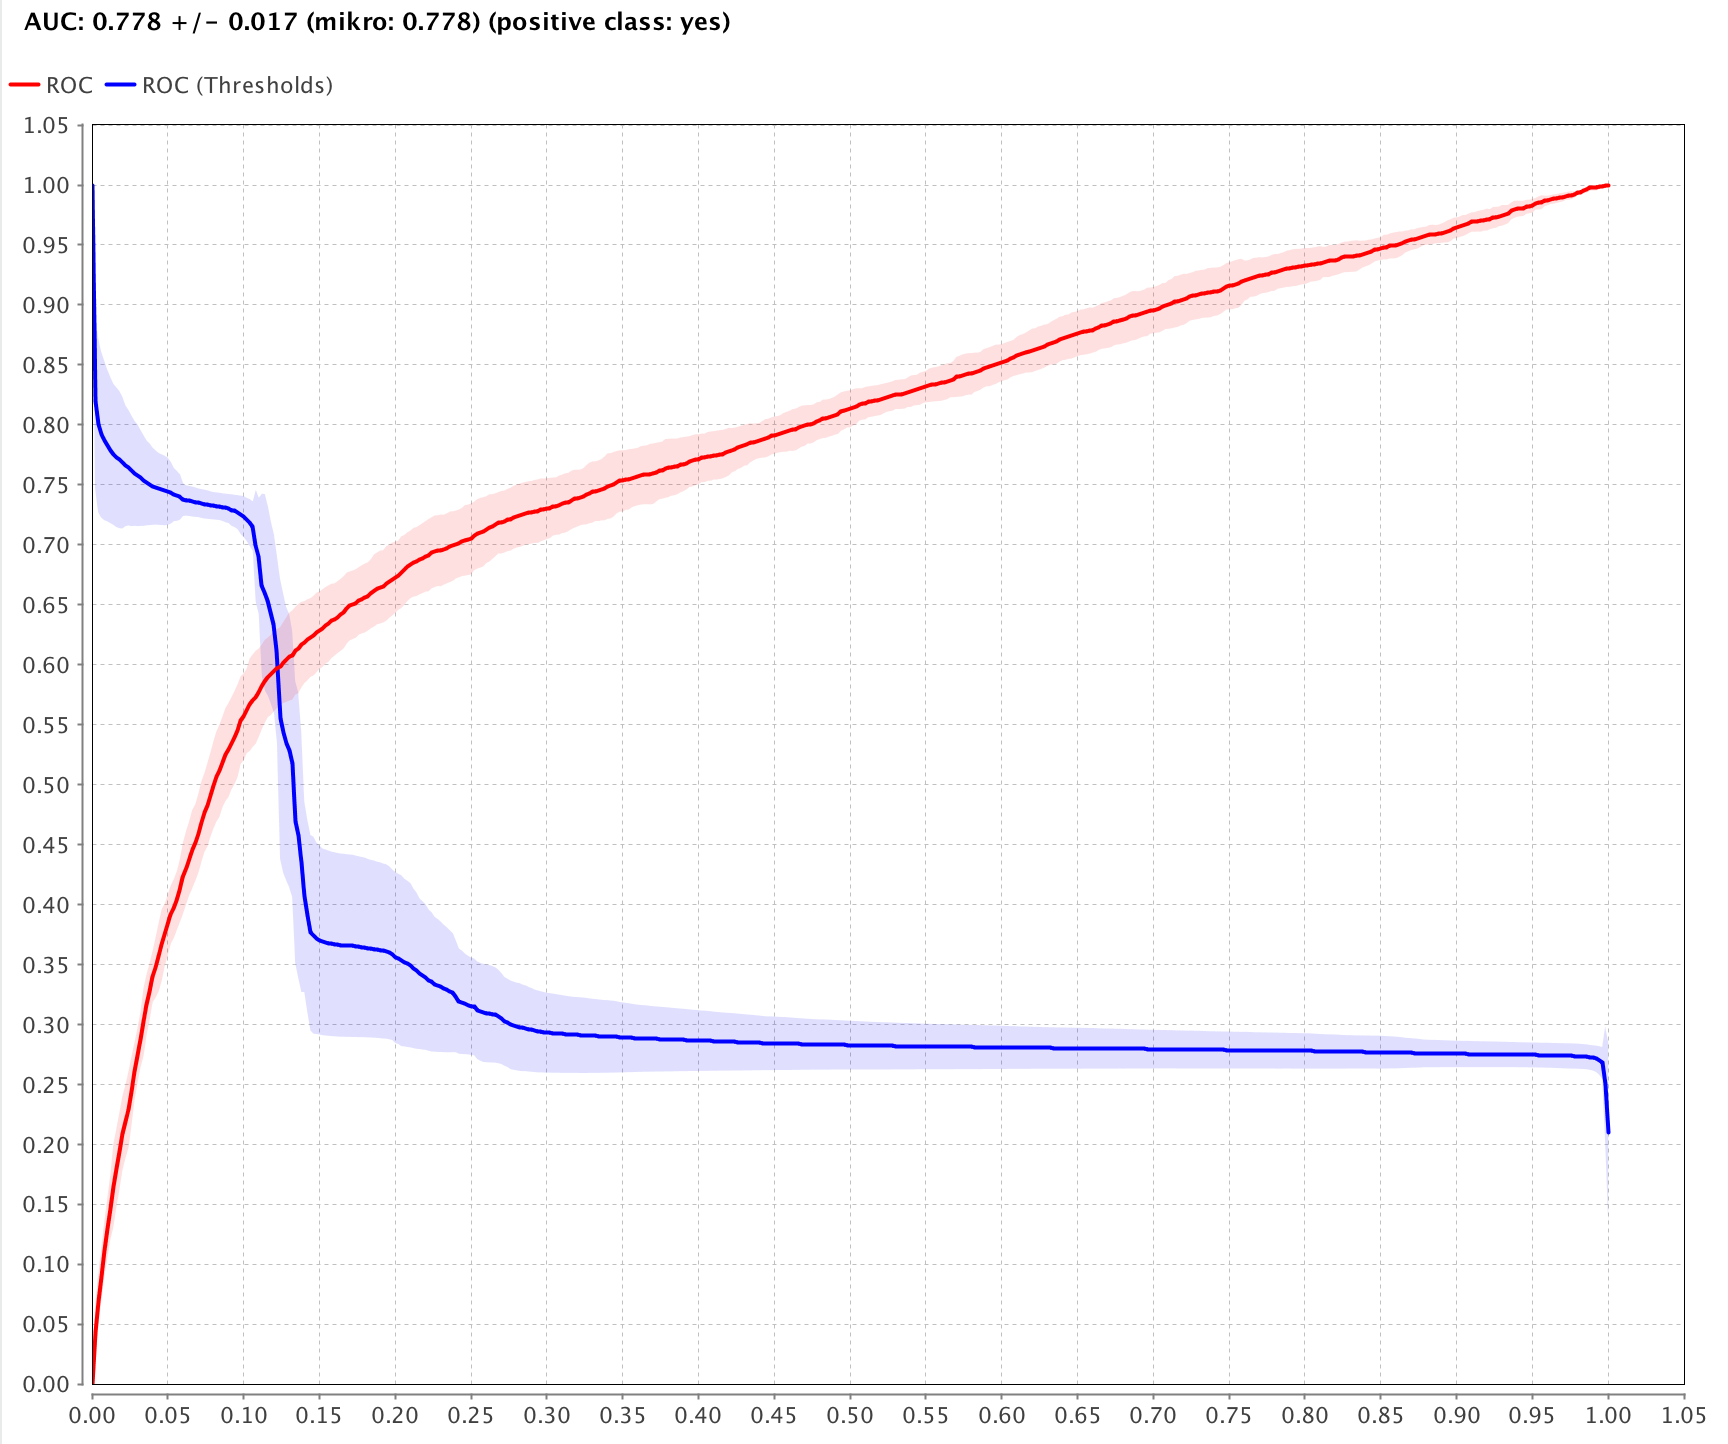
\includegraphics[width = \textwidth, height = 0.5\textheight, keepaspectratio]{svm-roc}}
\end{figure}

\begin{figure}[!t]
  \tbl{Options used in configuring the neural network.}{
    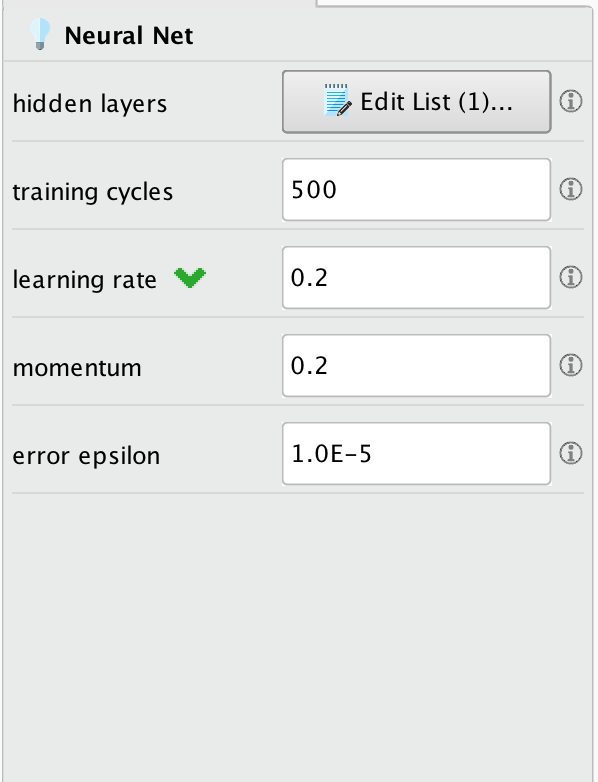
\includegraphics[width = \textwidth, height = 0.4\textheight, keepaspectratio]{nn-opt}}
\end{figure}

\begin{figure}[!t]
  \tbl{AUROC for the predictions made by the neural network.}{
    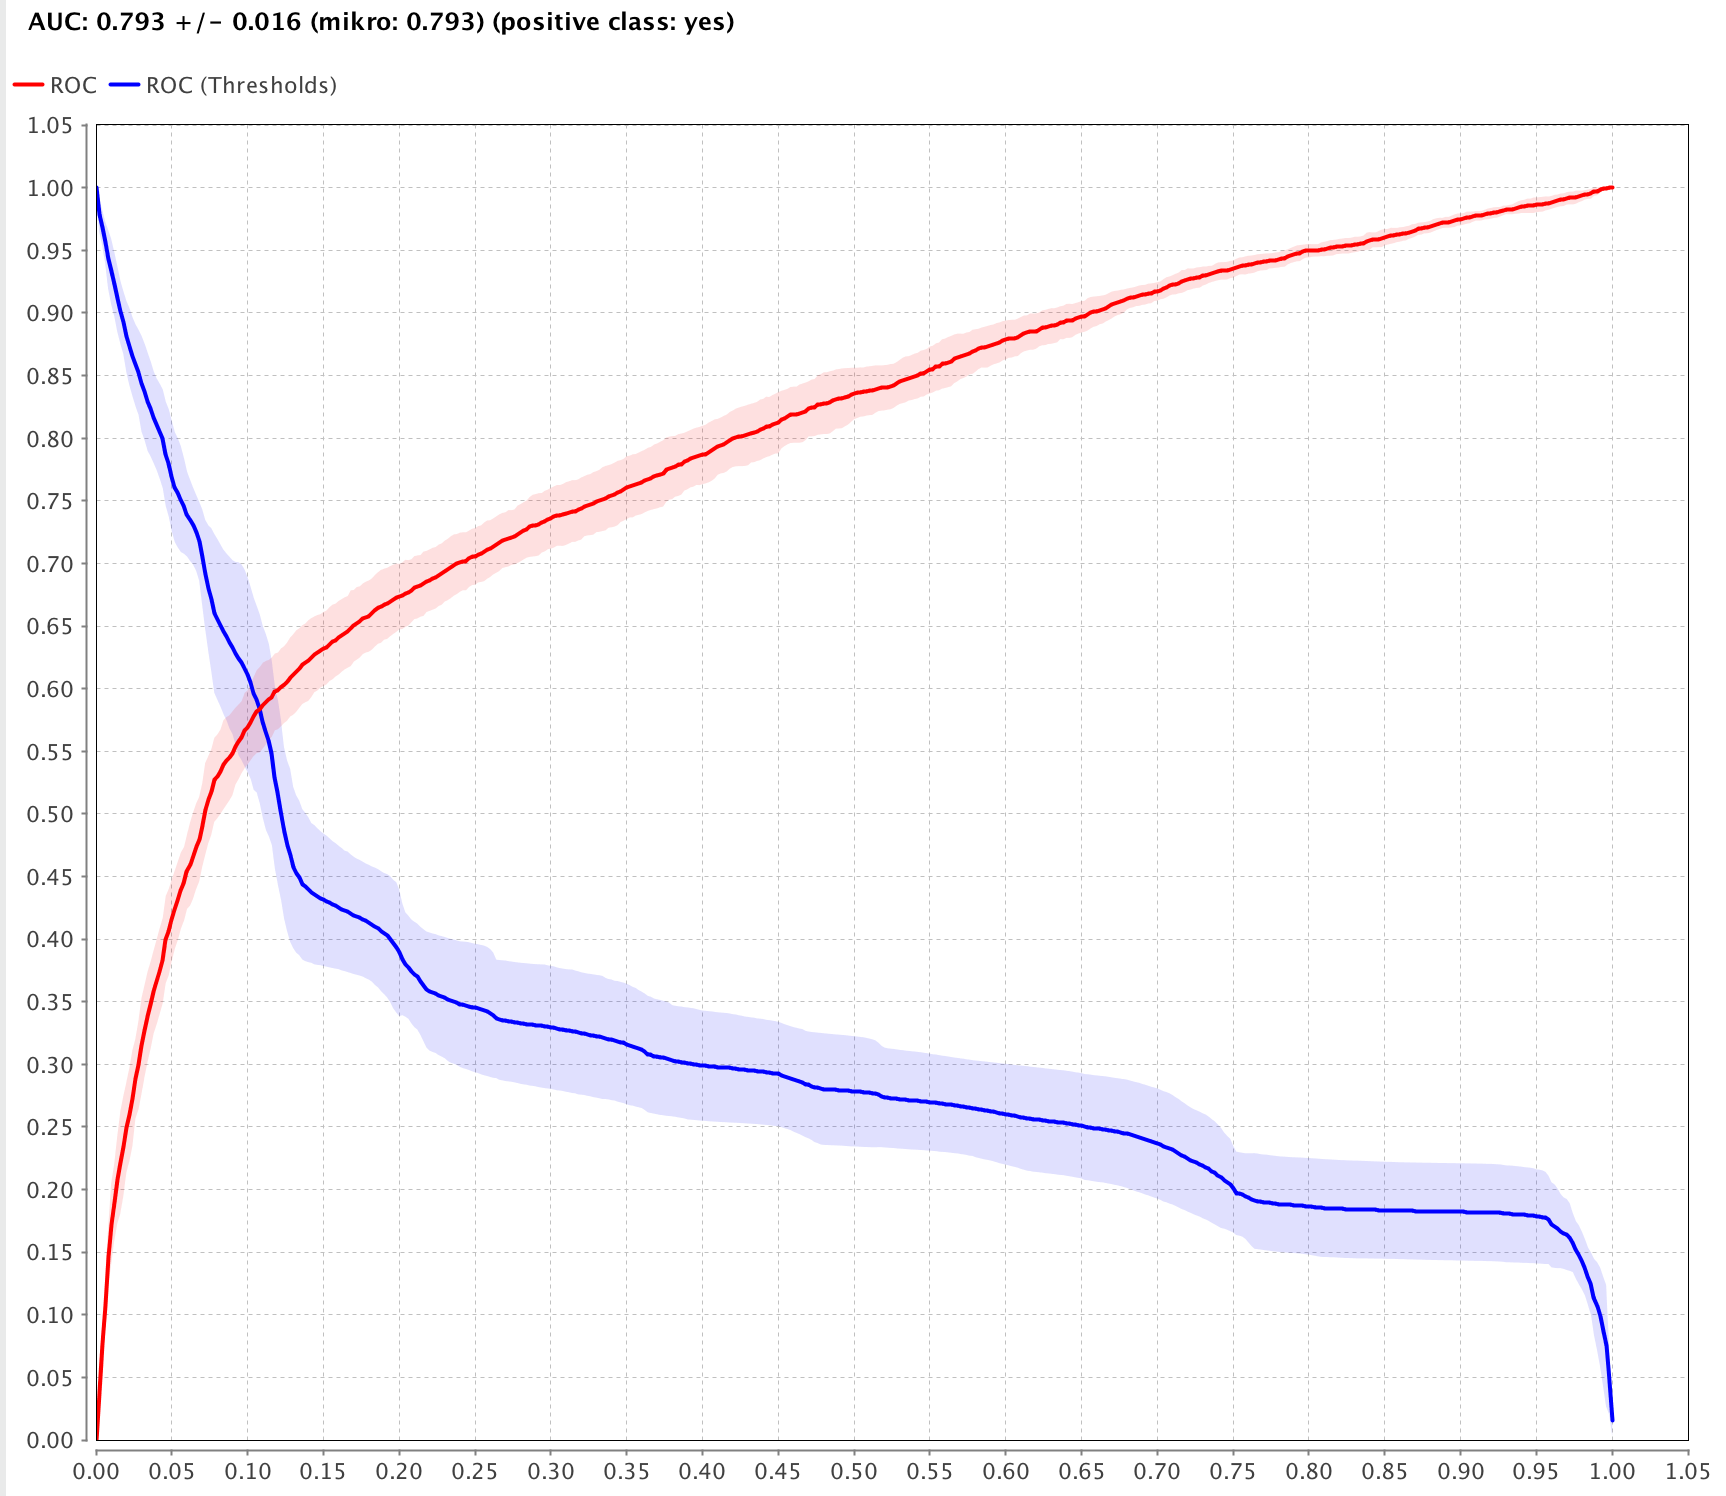
\includegraphics[width = \textwidth, height = 0.5\textheight, keepaspectratio]{nn-roc}}
\end{figure}

\begin{figure}[!t]
  \tbl{Options used in configuring the random forest.}{
    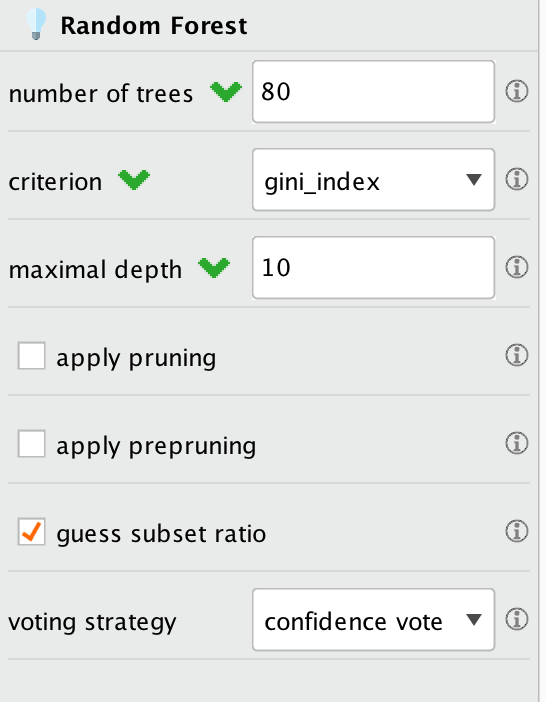
\includegraphics[width = \textwidth, height = 0.4\textheight, keepaspectratio]{rf-opt}}
\end{figure}

\begin{figure}[!t]
  \tbl{AUROC for the predictions made by the random forest.}{
    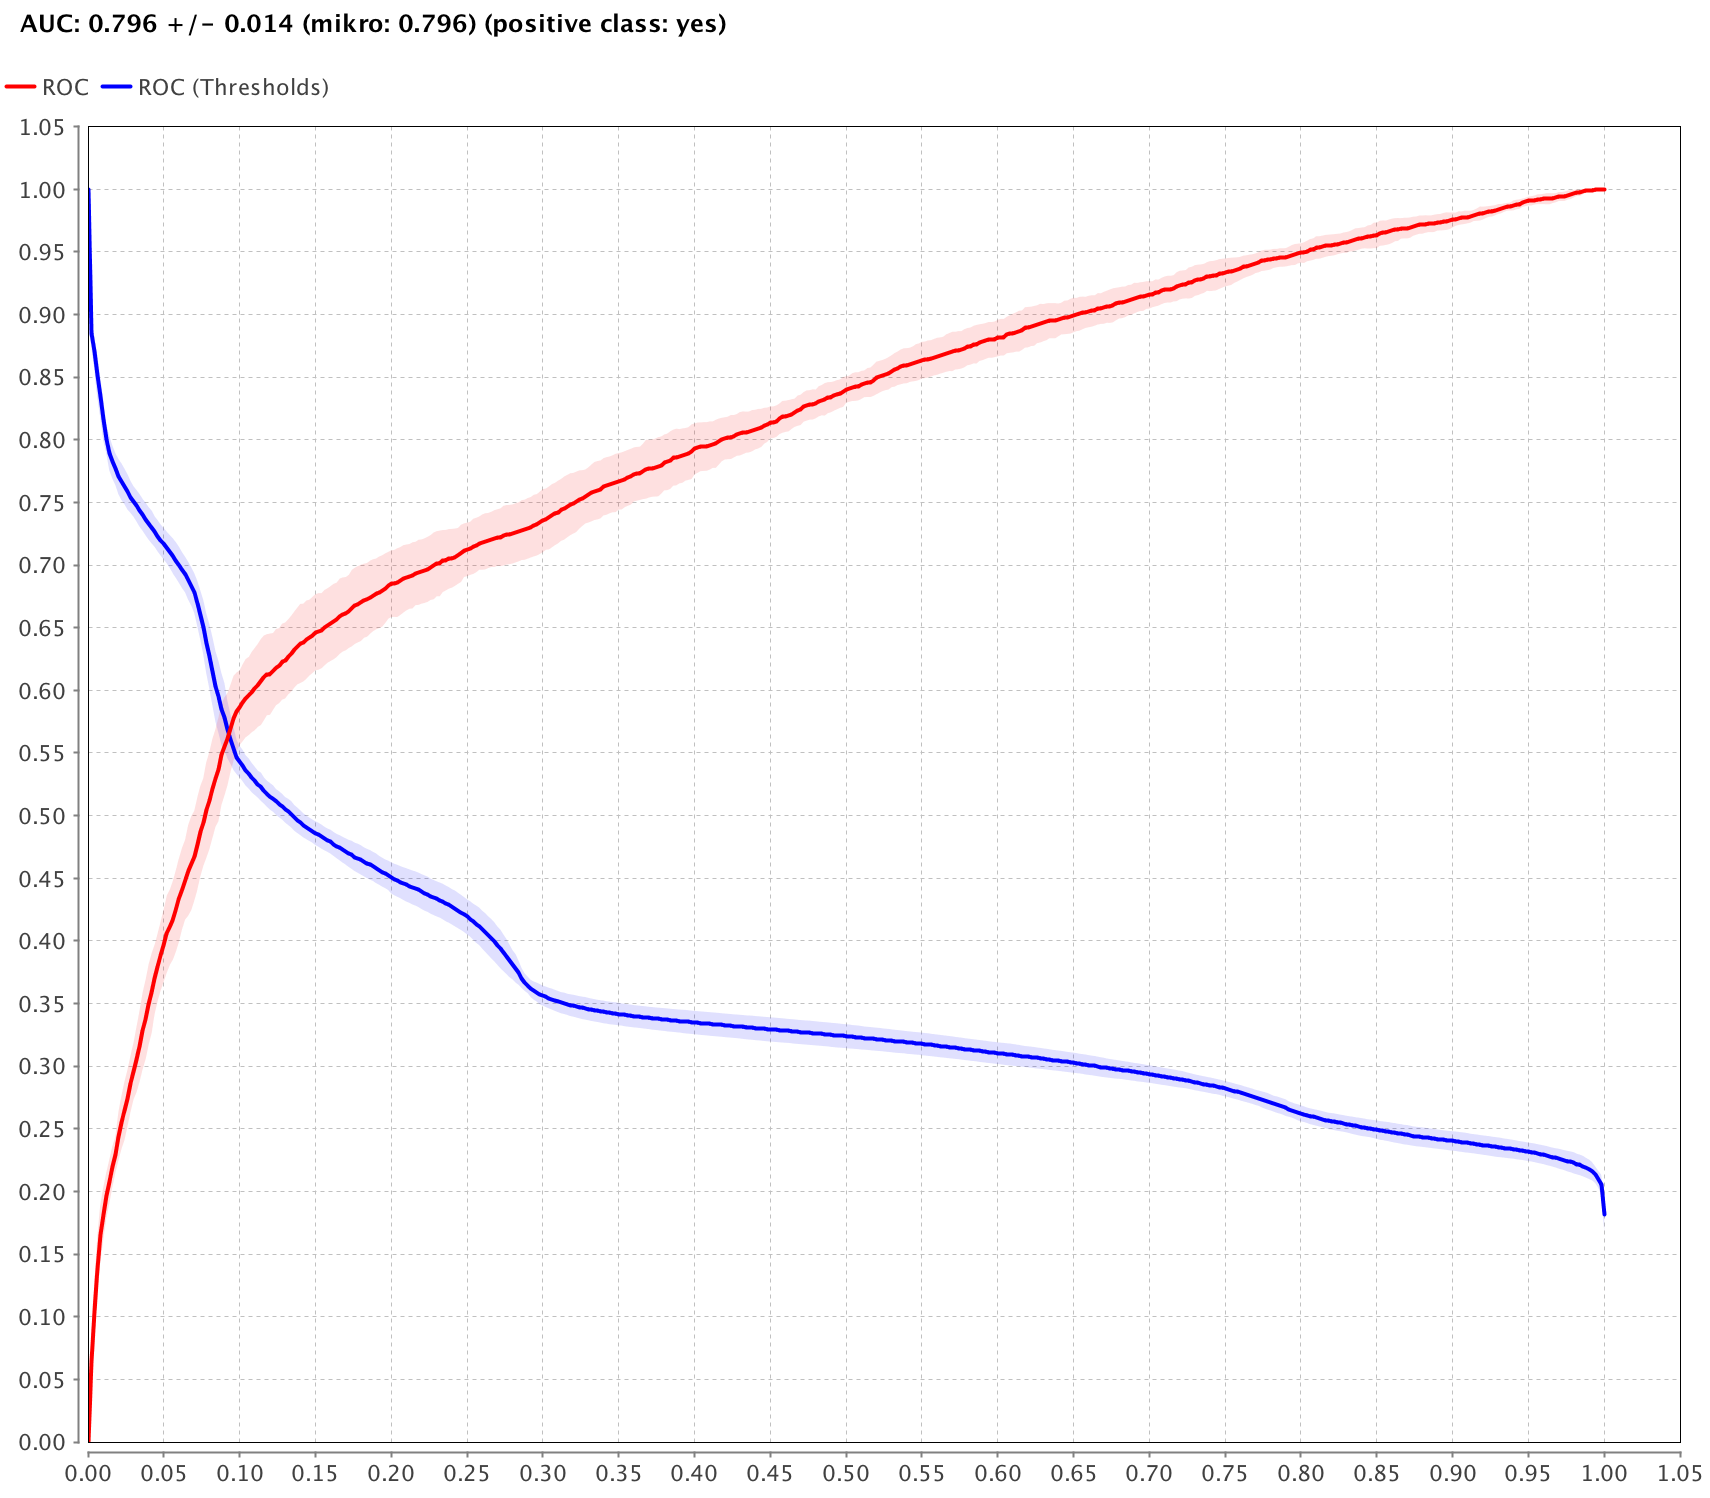
\includegraphics[width = \textwidth, height = 0.5\textheight, keepaspectratio]{rf-roc}}
\end{figure}

\begin{figure}[!t]
  \tbl{Text representation of the first tree generated by the random forest
    model, trimmed for brevity.}{}
    \begin{verbatim}
nr.employed > 5087.500
|   nr.employed > 5137.500
|   |   nr.employed > 5193
|   |   |   nr.employed > 5211.500: no (no=1950, yes=844)
|   |   |   nr.employed ≤ 5211.500
|   |   |   |   pdays > 5.500
|   |   |   |   |   pdays > 502.500: no (no=436, yes=234)
|   |   |   |   |   pdays ≤ 502.500: no (no=2, yes=1)
|   |   |   |   pdays ≤ 5.500
|   |   |   |   |   pdays > 4.500: yes (no=1, yes=3)
|   |   |   |   |   pdays ≤ 4.500: no (no=1, yes=0)
|   |   nr.employed ≤ 5193
|   |   |   nr.employed > 5183.500: no (no=1005, yes=230)
|   |   |   nr.employed ≤ 5183.500: no (no=5, yes=1)
|   nr.employed ≤ 5137.500
|   |   pdays > 11.500
|   |   |   pdays > 505.500: yes (no=912, yes=1003)
|   |   |   pdays ≤ 505.500: yes (no=4, yes=6)
|   |   pdays ≤ 11.500
|   |   |   pdays > 8
|   |   |   |   pdays > 10.500: yes (no=0, yes=11)
|   |   |   |   pdays ≤ 10.500
|   |   |   |   |   pdays > 9.500: yes (no=7, yes=13)
|   |   |   |   |   pdays ≤ 9.500: yes (no=1, yes=5)
|   |   |   pdays ≤ 8
|   |   |   |   pdays > 1.500
|   |   |   |   |   pdays > 2.500
|   |   |   |   |   |   pdays > 6.500: yes (no=0, yes=6)
|   |   |   |   |   |   pdays ≤ 6.500
|   |   |   |   |   |   |   pdays > 5.500: yes (no=2, yes=16)
|   |   |   |   |   |   |   pdays ≤ 5.500
|   |   |   |   |   |   |   |   pdays > 4: yes (no=0, yes=1)
|   |   |   |   |   |   |   |   pdays ≤ 4: yes (no=4, yes=35)
|   |   |   |   |   pdays ≤ 2.500: yes (no=0, yes=17)
|   |   |   |   pdays ≤ 1.500
|   |   |   |   |   pdays > 0.500: no (no=1, yes=1)
|   |   |   |   |   pdays ≤ 0.500: yes (no=0, yes=1)
nr.employed ≤ 5087.500
|   nr.employed > 5012.500
|   |   campaign > 5.500: yes (no=0, yes=20)
|   |   campaign ≤ 5.500
|   |   |   campaign > 2.500
|   |   |   |   nr.employed > 5049.500
|   |   |   |   |   campaign > 3.500
|   |   |   |   |   |   campaign > 4.500: yes (no=1, yes=6)
|   |   |   |   |   |   campaign ≤ 4.500: yes (no=5, yes=20)
|   |   |   |   |   campaign ≤ 3.500: yes (no=21, yes=55)
|   |   |   |   nr.employed ≤ 5049.500
|   |   |   |   |   campaign > 3.500
|   |   |   |   |   |   campaign > 4.500: yes (no=3, yes=6)
|   |   |   |   |   |   campaign ≤ 4.500
|   |   |   |   |   |   |   nr.employed > 5020: yes (no=1, yes=2)
|   |   |   |   |   |   |   nr.employed ≤ 5020: yes (no=3, yes=8)
|   |   |   |   |   campaign ≤ 3.500
|   |   |   |   |   |   nr.employed > 5020: yes (no=0, yes=9)
|   |   |   |   |   |   nr.employed ≤ 5020: yes (no=2, yes=28)
\end{verbatim}
\end{figure}

\begin{figure}[!t]
  \tbl{Text representation of a randomly selected tree generated by the random
    forest model.}{}
    \begin{verbatim}
euribor3m > 3.167
|   previous > 0.500: no (no=91, yes=31)
|   previous ≤ 0.500: no (no=3334, yes=1291)
euribor3m ≤ 3.167
|   previous > 1.500
|   |   previous > 5.500: no (no=3, yes=1)
|   |   previous ≤ 5.500
|   |   |   previous > 2.500
|   |   |   |   previous > 3.500
|   |   |   |   |   previous > 4.500: yes (no=0, yes=13)
|   |   |   |   |   previous ≤ 4.500: yes (no=3, yes=39)
|   |   |   |   previous ≤ 3.500: yes (no=16, yes=119)
|   |   |   previous ≤ 2.500: yes (no=63, yes=334)
|   previous ≤ 1.500
|   |   previous > 0.500: yes (no=377, yes=874)
|   |   previous ≤ 0.500: yes (no=813, yes=1878)
\end{verbatim}
\end{figure}

\begin{figure}[!t]
  \tbl{Text representation of a randomly selected tree generated by the random
    forest model, trimmed for brevity.}{}
    \begin{verbatim}
nr.employed > 5087.500
|   euribor3m > 3.308
|   |   euribor3m > 4.889
|   |   |   campaign > 11.500
|   |   |   |   euribor3m > 4.963
|   |   |   |   |   euribor3m > 4.965
|   |   |   |   |   |   euribor3m > 4.966: no (no=12, yes=1)
|   |   |   |   |   |   euribor3m ≤ 4.966: no (no=1, yes=0)
|   |   |   |   |   euribor3m ≤ 4.965: no (no=6, yes=3)
|   |   |   |   euribor3m ≤ 4.963
|   |   |   |   |   euribor3m > 4.958
|   |   |   |   |   |   euribor3m > 4.962
|   |   |   |   |   |   |   euribor3m > 4.963: no (no=5, yes=0)
|   |   |   |   |   |   |   euribor3m ≤ 4.963: no (no=17, yes=1)
|   |   |   |   |   |   euribor3m ≤ 4.962: no (no=24, yes=0)
|   |   |   |   |   euribor3m ≤ 4.958
|   |   |   |   |   |   euribor3m > 4.953: no (no=1, yes=1)
|   |   |   |   |   |   euribor3m ≤ 4.953: no (no=1, yes=0)
|   |   |   campaign ≤ 11.500
|   |   |   |   euribor3m > 4.957
|   |   |   |   |   campaign > 2.500
|   |   |   |   |   |   campaign > 5.500
|   |   |   |   |   |   |   campaign > 9.500
|   |   |   |   |   |   |   |   campaign > 10.500: no (no=13, yes=7)
|   |   |   |   |   |   |   |   campaign ≤ 10.500: no (no=19, yes=5)
|   |   |   |   |   |   |   campaign ≤ 9.500
|   |   |   |   |   |   |   |   campaign > 6.500: no (no=52, yes=38)
|   |   |   |   |   |   |   |   campaign ≤ 6.500: no (no=45, yes=26)
|   |   |   |   |   |   campaign ≤ 5.500
|   |   |   |   |   |   |   campaign > 3.500
|   |   |   |   |   |   |   |   campaign > 4.500: no (no=68, yes=34)
|   |   |   |   |   |   |   |   campaign ≤ 4.500: no (no=141, yes=61)
|   |   |   |   |   |   |   campaign ≤ 3.500: no (no=251, yes=125)
|   |   |   |   |   campaign ≤ 2.500
|   |   |   |   |   |   campaign > 1.500: no (no=415, yes=177)
|   |   |   |   |   |   campaign ≤ 1.500: no (no=630, yes=261)
|   |   |   |   euribor3m ≤ 4.957
|   |   |   |   |   euribor3m > 4.915
|   |   |   |   |   |   euribor3m > 4.920
|   |   |   |   |   |   |   euribor3m > 4.941
|   |   |   |   |   |   |   |   euribor3m > 4.957: no (no=64, yes=54)
|   |   |   |   |   |   |   |   euribor3m ≤ 4.957: no (no=26, yes=17)
|   |   |   |   |   |   |   euribor3m ≤ 4.941: yes (no=0, yes=5)
|   |   |   |   |   |   euribor3m ≤ 4.920: no (no=4, yes=1)
|   |   |   |   |   euribor3m ≤ 4.915: yes (no=0, yes=3)
\end{verbatim}
\end{figure}

\begin{figure}[!t]
  \tbl{Text representation of the last tree generated by the random forest
    model, trimmed for brevity.}{}
    \begin{verbatim}
emp.var.rate > -0.650
|   contact = cellular
|   |   default = no
|   |   |   emp.var.rate > 0.650: no (no=949, yes=484)
|   |   |   emp.var.rate ≤ 0.650
|   |   |   |   emp.var.rate > -0.150: no (no=380, yes=167)
|   |   |   |   emp.var.rate ≤ -0.150: no (no=1, yes=0)
|   |   default = unknown
|   |   |   emp.var.rate > 0.650: no (no=315, yes=140)
|   |   |   emp.var.rate ≤ 0.650: no (no=45, yes=24)
|   |   default = yes: no (no=1, yes=0)
|   contact = telephone
|   |   emp.var.rate > 0.500
|   |   |   campaign > 15.500: no (no=35, yes=0)
|   |   |   campaign ≤ 15.500
|   |   |   |   campaign > 5.500
|   |   |   |   |   emp.var.rate > 1.250
|   |   |   |   |   |   campaign > 8.500
|   |   |   |   |   |   |   campaign > 12.500
|   |   |   |   |   |   |   |   campaign > 14.500: no (no=4, yes=2)
|   |   |   |   |   |   |   |   campaign ≤ 14.500: no (no=3, yes=2)
|   |   |   |   |   |   |   campaign ≤ 12.500
|   |   |   |   |   |   |   |   campaign > 9.500: no (no=20, yes=3)
|   |   |   |   |   |   |   |   campaign ≤ 9.500: no (no=8, yes=4)
|   |   |   |   |   |   campaign ≤ 8.500
|   |   |   |   |   |   |   campaign > 6.500
|   |   |   |   |   |   |   |   campaign > 7.500: no (no=9, yes=8)
|   |   |   |   |   |   |   |   campaign ≤ 7.500: yes (no=6, yes=8)
|   |   |   |   |   |   |   campaign ≤ 6.500: no (no=17, yes=15)
|   |   |   |   |   emp.var.rate ≤ 1.250: no (no=69, yes=12)
|   |   |   |   campaign ≤ 5.500
|   |   |   |   |   campaign > 4.500: no (no=79, yes=14)
|   |   |   |   |   campaign ≤ 4.500
|   |   |   |   |   |   campaign > 3.500: no (no=121, yes=30)
|   |   |   |   |   |   campaign ≤ 3.500
|   |   |   |   |   |   |   campaign > 1.500
|   |   |   |   |   |   |   |   campaign > 2.500: no (no=220, yes=67)
|   |   |   |   |   |   |   |   campaign ≤ 2.500: no (no=443, yes=137)
|   |   |   |   |   |   |   campaign ≤ 1.500: no (no=612, yes=168)
|   |   emp.var.rate ≤ 0.500
|   |   |   campaign > 1.500
|   |   |   |   default = no
|   |   |   |   |   campaign > 3.500: no (no=7, yes=0)
|   |   |   |   |   campaign ≤ 3.500
|   |   |   |   |   |   campaign > 2.500: no (no=1, yes=1)
|   |   |   |   |   |   campaign ≤ 2.500: no (no=4, yes=0)
|   |   |   |   default = unknown
|   |   |   |   |   campaign > 2.500: no (no=2, yes=0)
|   |   |   |   |   campaign ≤ 2.500: yes (no=0, yes=2)
|   |   |   campaign ≤ 1.500: yes (no=21, yes=74)
\end{verbatim}
\end{figure}

% Decision tree baseline
% Decision tree improved
% SVM
% Neural Net
% Random forest
% Other classification models and etc.

% Conclusions:
% 2/3 recall for 1/4 calls.
% call 160,000 people for 8/3 revenue.
% Plot duration, show that it is low for no responses.
% Suggest models that can vary sampling to produce more yes results.
% Further study: different data, better sampling, different classifiers.

\end{document}
% End of v2-acmsmall-sample.tex (March 2012) - Gerry Murray, ACM


